% Options for packages loaded elsewhere
\PassOptionsToPackage{unicode}{hyperref}
\PassOptionsToPackage{hyphens}{url}
%
\documentclass[
]{article}
\usepackage{amsmath,amssymb}
\usepackage{iftex}
\ifPDFTeX
  \usepackage[T1]{fontenc}
  \usepackage[utf8]{inputenc}
  \usepackage{textcomp} % provide euro and other symbols
\else % if luatex or xetex
  \usepackage{unicode-math} % this also loads fontspec
  \defaultfontfeatures{Scale=MatchLowercase}
  \defaultfontfeatures[\rmfamily]{Ligatures=TeX,Scale=1}
\fi
\usepackage{lmodern}
\ifPDFTeX\else
  % xetex/luatex font selection
\fi
% Use upquote if available, for straight quotes in verbatim environments
\IfFileExists{upquote.sty}{\usepackage{upquote}}{}
\IfFileExists{microtype.sty}{% use microtype if available
  \usepackage[]{microtype}
  \UseMicrotypeSet[protrusion]{basicmath} % disable protrusion for tt fonts
}{}
\makeatletter
\@ifundefined{KOMAClassName}{% if non-KOMA class
  \IfFileExists{parskip.sty}{%
    \usepackage{parskip}
  }{% else
    \setlength{\parindent}{0pt}
    \setlength{\parskip}{6pt plus 2pt minus 1pt}}
}{% if KOMA class
  \KOMAoptions{parskip=half}}
\makeatother
\usepackage{xcolor}
\usepackage[margin=1in]{geometry}
\usepackage{graphicx}
\makeatletter
\def\maxwidth{\ifdim\Gin@nat@width>\linewidth\linewidth\else\Gin@nat@width\fi}
\def\maxheight{\ifdim\Gin@nat@height>\textheight\textheight\else\Gin@nat@height\fi}
\makeatother
% Scale images if necessary, so that they will not overflow the page
% margins by default, and it is still possible to overwrite the defaults
% using explicit options in \includegraphics[width, height, ...]{}
\setkeys{Gin}{width=\maxwidth,height=\maxheight,keepaspectratio}
% Set default figure placement to htbp
\makeatletter
\def\fps@figure{htbp}
\makeatother
\setlength{\emergencystretch}{3em} % prevent overfull lines
\providecommand{\tightlist}{%
  \setlength{\itemsep}{0pt}\setlength{\parskip}{0pt}}
\setcounter{secnumdepth}{5}
\newlength{\cslhangindent}
\setlength{\cslhangindent}{1.5em}
\newlength{\csllabelwidth}
\setlength{\csllabelwidth}{3em}
\newlength{\cslentryspacingunit} % times entry-spacing
\setlength{\cslentryspacingunit}{\parskip}
\newenvironment{CSLReferences}[2] % #1 hanging-ident, #2 entry spacing
 {% don't indent paragraphs
  \setlength{\parindent}{0pt}
  % turn on hanging indent if param 1 is 1
  \ifodd #1
  \let\oldpar\par
  \def\par{\hangindent=\cslhangindent\oldpar}
  \fi
  % set entry spacing
  \setlength{\parskip}{#2\cslentryspacingunit}
 }%
 {}
\usepackage{calc}
\newcommand{\CSLBlock}[1]{#1\hfill\break}
\newcommand{\CSLLeftMargin}[1]{\parbox[t]{\csllabelwidth}{#1}}
\newcommand{\CSLRightInline}[1]{\parbox[t]{\linewidth - \csllabelwidth}{#1}\break}
\newcommand{\CSLIndent}[1]{\hspace{\cslhangindent}#1}
\usepackage{setspace}\doublespacing
\usepackage[fontsize=12pt]{scrextend}
\usepackage[left]{lineno}
\usepackage[labelformat=empty]{caption}
\usepackage{longtable}
\usepackage{booktabs}
\usepackage{booktabs}
\usepackage{longtable}
\usepackage{array}
\usepackage{multirow}
\usepackage{wrapfig}
\usepackage{float}
\usepackage{colortbl}
\usepackage{pdflscape}
\usepackage{tabu}
\usepackage{threeparttable}
\usepackage{threeparttablex}
\usepackage[normalem]{ulem}
\usepackage{makecell}
\usepackage{xcolor}
\ifLuaTeX
  \usepackage{selnolig}  % disable illegal ligatures
\fi
\IfFileExists{bookmark.sty}{\usepackage{bookmark}}{\usepackage{hyperref}}
\IfFileExists{xurl.sty}{\usepackage{xurl}}{} % add URL line breaks if available
\urlstyle{same}
\hypersetup{
  hidelinks,
  pdfcreator={LaTeX via pandoc}}

\author{}
\date{\vspace{-2.5em}}

\begin{document}

\hypertarget{title-page}{%
\section{Title Page}\label{title-page}}

\textbf{Sensory processing in humans and mice fluctuates between
external and internal modes}\\
\strut \\

\textbf{Authors}:

Veith Weilnhammer\(^{1,2, 3, *}\), Heiner Stuke\(^{1,2}\), Kai
Standvoss\(^{1}\), Philipp Sterzer\(^{4}\)\\
\strut \\
\textbf{Affiliations}:

\(^{1}\) Department of Psychiatry, Charité-Universitätsmedizin Berlin,
corporate member of Freie Universität Berlin and Humboldt-Universität zu
Berlin, Berlin, Germany\\
\(^{2}\) Berlin Institute of Health, Charité-Universitätsmedizin Berlin
and Max Delbrück Center, Berlin, Germany\\
\(^{3}\) Helen Wills Neuroscience Institute, University of California
Berkeley, Berkeley, California, United States of America\\
\(^{4}\) Department of Psychiatry (UPK), University of Basel, Basel, 
Switzerland\\
\strut \

* veith.weilnhammer@gmail.com

\newpage

\hypertarget{abstract}{%
\section{Abstract}\label{abstract}}

Perception is known to cycle through periods of enhanced and reduced
sensitivity to external information. Here, we asked whether such slow
fluctuations arise as a noise-related epiphenomenon of limited
processing capacity or, alternatively, represent a structured mechanism
of perceptual inference. Using two large-scale datasets, we found that
humans and mice alternate between externally- and internally-oriented
modes of sensory analysis. During external mode, perception aligns more
closely with the external sensory information, whereas internal mode is
characterized by enhanced biases toward perceptual history.
Computational modeling indicated that dynamic changes in mode are
enabled by two interlinked factors: (i), the integration of subsequent
inputs over time and, (ii), slow anti-phase oscillations in the
perceptual impact of external sensory information versus internal
predictions that are provided by perceptual history. We propose that
between-mode fluctuations generate unambiguous error signals that enable
optimal inference in volatile environments.

\hypertarget{one-sentence-summary}{%
\section{One sentence summary}\label{one-sentence-summary}}

Humans and mice fluctuate between external and internal modes of sensory
processing.

\hfill\break

\newpage

\hypertarget{introduction}{%
\section{Introduction}\label{introduction}}

The capacity to respond to changes in the environment is a defining
feature of life\textsuperscript{1--3}. Intriguingly, the ability of
living things to process their surroundings fluctuates considerably over
time\textsuperscript{4,5}. In humans and mice,
perception\textsuperscript{6--12}, cognition\textsuperscript{13} and
memory\textsuperscript{14} cycle through prolonged periods of enhanced
and reduced sensitivity to external information, suggesting that the
brain detaches from the world in recurring intervals that last from
milliseconds to seconds and even minutes\textsuperscript{4}. Yet
breaking from external information is risky, as swift responses to the
environment are often crucial to survival.

What could be the reason for these fluctuations in perceptual
performance\textsuperscript{11}? First, periodic fluctuations in the
ability to parse external information\textsuperscript{11,15,16} may
arise simply due to bandwidth limitations and noise. Second, it may be
advantageous to actively reduce the costs of neural processing by
seeking sensory information only in recurring
intervals\textsuperscript{17}, otherwise relying on random or
stereotypical responses to the external world. Third, spending time away
from the ongoing stream of sensory inputs may also reflect a functional
strategy that facilitates flexible behavior and
learning\textsuperscript{18}: Intermittently relying more strongly on
information acquired from past experiences may enable agents to build up
stable internal predictions about the environment despite an ongoing
stream of external sensory signals\textsuperscript{19}. By the same
token, recurring intervals of enhanced sensitivity to external
information may help to detect changes in both the state of the
environment and the amount of noise that is inherent in sensory
encoding\textsuperscript{19}.

In this work, we sought to elucidate whether periodicities in the
sensitivity to external information represent an epiphenomenon of
limited processing capacity or, alternatively, result from a structured
and adaptive mechanism of perceptual inference. To this end, we analyzed
two large-scale datasets on perceptual decision-making in
humans\textsuperscript{20} and mice\textsuperscript{21}. When less
sensitive to external stimulus information, humans and mice did not
behave more randomly, but showed stronger serial dependencies in their
perceptual choices\textsuperscript{22--33}. These serial dependencies
may be understood as driven by internal predictions that reflect the
autocorrelation of natural environments\textsuperscript{34} and bias
perception toward preceding experiences\textsuperscript{30,31,35}.
Computational modeling indicated that ongoing changes in perceptual
performance may be driven by systematic fluctuations between externally-
and internally-oriented \emph{modes} of sensory analysis. We suggest
that such \emph{bimodal inference} may help to build stable internal
representations of the sensory environment despite an ongoing stream of
sensory information.

\hypertarget{results}{%
\section{Results}\label{results}}

\hypertarget{human-perception-fluctuates-between-epochs-of-enhanced-and-reduced-sensitivity-to-external-information}{%
\subsection{Human perception fluctuates between epochs of enhanced and
reduced sensitivity to external
information}\label{human-perception-fluctuates-between-epochs-of-enhanced-and-reduced-sensitivity-to-external-information}}

We began by selecting 66 studies from the Confidence
Database\textsuperscript{20} that investigated how human participants (N
= 4317) perform binary perceptual decisions (Fig 1A; see Methods for
details on inclusion criteria). As a metric for perceptual performance
(i.e., the sensitivity to external sensory information), we asked
whether the participant's response and the presented stimulus matched
(\emph{stimulus-congruent} choices) or differed from each other
(\emph{stimulus-incongruent} choices; Figs 1B and 1C) in a total of
\(21.05\) million trials.

In a first step, we asked whether the ability to accurately perceive
sensory stimuli is constant over time or, alternatively, fluctuates in
periods of enhanced and reduced sensitivity to external information. We
found perception to be stimulus-congruent in 73.46\% ± 0.15\% of trials
(mean ± standard error of the mean; Fig 2A), which was highly
consistent across the selected studies (S1A Fig). In
line with previous work\textsuperscript{8}, we found that the
probability of stimulus-congruence was not independent across successive
trials: At the group level, stimulus-congruent perceptual choices were
significantly autocorrelated for up to 15 trials (Fig 2B),
controlling for task difficulty and the sequence of presented stimuli
(S2 Fig).

At the level of individual participants, the autocorrelation of
stimulus-congruence exceeded the respective autocorrelation of randomly
permuted data within an interval of \(3.24\) ±
\(\ensuremath{2.39\times 10^{-3}}\) trials (Fig 2C). In other words,
if a participant's experience was congruent (or incongruent) with the
external stimulus information at a given trial, her perception was more
likely to remain stimulus-congruent (or -incongruent) for approximately
3 trials into the future. The autocorrelation of stimulus-congruence was
corroborated by logistic regression models that successfully predicted
the stimulus-congruence of perception at the index trial \(t = 0\) from
the stimulus-congruence at the preceding trials within a lag of 16
trials (S3 Fig).

These results confirm that the ability to process sensory signals is not
constant over time but unfolds in multi-trial epochs of enhanced and
reduced sensitivity to external information\textsuperscript{8}. As a
consequence of this autocorrelation, the dynamic probability of
stimulus-congruent perception (i.e., computed in sliding windows of ± 5
trials; Fig 1C) fluctuated considerably within participants (average
minimum: 35.46\% ± 0.22\%, maximum: 98.27\% ± 0.07\%). In line with
previous findings\textsuperscript{9}, such fluctuations in the
sensitivity to external information had a power density that was
inversely proportional to the frequency in the slow
spectrum\textsuperscript{11} (power \textasciitilde{} 1/\(f^\beta\),
\(\beta\) = \(-1.32\) ± \(\ensuremath{3.14\times 10^{-3}}\),
T(\(\ensuremath{1.84\times 10^{5}}\)) = \(-419.48\), p < \(\ensuremath{2.2\times 10^{-308}}\); Fig
2D). This feature, which is also known as a \emph{1/f power
law}\textsuperscript{36,37}, represents a characteristic of scale-free
fluctuations in complex dynamic systems such as the
brain\textsuperscript{38} and the cognitive processes it
entertains\textsuperscript{9,10,13,39,40}.

\hypertarget{humans-fluctuate-between-external-and-internal-modes-of-sensory-processing}{%
\subsection{Humans fluctuate between external and internal modes of
sensory
processing}\label{humans-fluctuate-between-external-and-internal-modes-of-sensory-processing}}

In a second step, we sought to explain why perception cycles through
periods of enhanced and reduced sensitivity to external
information\textsuperscript{4}. We reasoned that observers may
intermittently rely more strongly on internal information, i.e., on
predictions about the environment that are constructed from previous
experiences\textsuperscript{19,31}.

In perception, \emph{serial dependencies} represent one of the most
basic internal predictions that cause perceptual decisions to be
systematically biased toward preceding choices\textsuperscript{22--33}.
Such effects of perceptual history mirror the continuity of the external
world, in which the recent past often predicts the near
future\textsuperscript{30,31,34,35,41}. Therefore, as a metric for the
perceptual impact of internal information, we computed whether the
participant's response at a given trial matched or differed from her
response at the preceding trial (\emph{history-congruent} and
\emph{history-incongruent perception}, respectively; Figs 1B and 1C).

First, we confirmed that perceptual history played a significant role in
perception despite the ongoing stream of external information. With a
global average of 52.7\% ± 0.12\% history-congruent trials, we found a
small but highly significant perceptual bias towards preceding
experiences (\(\beta\) = \(16.18\) ± \(1.07\),
T(\(\ensuremath{1.09\times 10^{3}}\)) = \(15.07\), p =
\(\ensuremath{10^{-46}}\); Fig 2A) that was largely consistent across
studies (S1B Fig) and more pronounced in participants who
were less sensitive to external sensory information (S1C Fig). Importantly, history-congruence was not a corollary of the sequence
of presented stimuli: History-congruent perceptual choices were more
frequent at trials when perception was stimulus-incongruent (56.03\% ±
0.2\%) as opposed to stimulus-congruent (51.77\% ± 0.11\%, \(\beta\) =
\(-4.26\) ± \(0.21\), T(\(\ensuremath{8.57\times 10^{3}}\)) =
\(-20.36\), p = \(\ensuremath{5.28\times 10^{-90}}\); Fig 2A, lower
panel). Despite being adaptive in autocorrelated real-world
environments\textsuperscript{19,34,35,42}, perceptual history thus
represented a source of bias in the randomized experimental designs
studied here\textsuperscript{24,28,30,31,43}. These serial biases were
effects of choice history, i.e., driven by the experiences reported at
the preceding trial, and could not be attributed to stimulus history,
i.e., to effects of the stimuli presented at the preceding trial
(S1 Text).

Second, we asked whether perception cycles through multi-trial epochs
during which perception is characterized by stronger or weaker biases
toward preceding experiences. In close analogy to stimulus-congruence,
we found history-congruence to be significantly autocorrelated for up to
21 trials (Fig 2B), while controlling for task difficulty and the
sequence of presented stimuli (S2 Fig). In individual
participants, the autocorrelation of history-congruence was elevated
above randomly permuted data for a lag of \(4.87\) ±
\(\ensuremath{3.36\times 10^{-3}}\) trials (Fig 2C), confirming that
the autocorrelation of history-congruence was not only a group-level
phenomenon. The autocorrelation of history-congruence was corroborated
by logistic regression models that successfully predicted the
history-congruence of perception at an index trial \(t = 0\) from the
history-congruence at the preceding trials within a lag of 17 trials
(S3 Fig).

Third, we asked whether the impact of internal information fluctuates as
a scale-invariant process with a 1/f power law (i.e., the feature
typically associated with fluctuations in the sensitivity to external
information\textsuperscript{9,10,13,39,40}). The dynamic probability of
history-congruent perception (i.e., computed in sliding windows of ± 5
trials; Fig 1C) varied considerably over time, ranging between a
minimum of 12.77\% ± 0.14\% and a maximum 92.23\% ± 0.14\%. In analogy
to stimulus-congruence, we found that history-congruence fluctuated as
at power densities that were inversely proportional to the frequency in
the slow spectrum\textsuperscript{11} (power \textasciitilde{}
1/\(f^\beta\), \(\beta\) = \(-1.34\) ±
\(\ensuremath{3.16\times 10^{-3}}\),
T(\(\ensuremath{1.84\times 10^{5}}\)) = \(-423.91\), p < \(\ensuremath{2.2\times 10^{-308}}\); Fig
2D).

Finally, we ensured that fluctuations in stimulus- and
history-congruence are linked to each other. When perceptual choices
were less biased toward external information, participants relied more
strongly on internal information acquired from perceptual history (and
vice versa, \(\beta\) = \(-0.05\) ± \(\ensuremath{5.63\times 10^{-4}}\),
T(\(\ensuremath{2.1\times 10^{6}}\)) = \(-84.21\), p < \(\ensuremath{2.2\times 10^{-308}}\),
controlling for fluctuations in general response biases; S1 Text). Thus, while sharing the 1/f power law characteristic,
fluctuations in stimulus- and history-congruence were shifted against
each other by approximately half a cycle and showed a squared coherence
of \(6.49\) ± \(\ensuremath{2.07\times 10^{-3}}\)\% (Figs 2E and 2F; we
report the average phase and coherence for frequencies below 0.1
\(1/N_{trials}\); see Methods for details).

In sum, our analyses indicate that perceptual decisions may result from
a competition between external sensory signals with internal predictions
provided by perceptual history. We show that the impact of these
external and internal sources of information is not stable over time,
but fluctuates systematically, emitting overlapping autocorrelation
curves and antiphase 1/f profiles.

These links between stimulus- and history-congruence suggest that the
fluctuations in the impact of external and internal information may be
generated by a unifying mechanism that causes perception to alternate
between two opposing \emph{modes}\textsuperscript{18} (Fig 1D):
During \emph{external mode}, perception is more strongly driven by the
available external stimulus information. Conversely, during
\emph{internal mode}, participants rely more heavily on internal
predictions that are implicitly provided by preceding perceptual
experiences. The fluctuations in the degree of bias toward external
versus internal information created by such \emph{bimodal inference} may
thus provide a novel explanation for ongoing fluctuations in the
sensitivity to external information\textsuperscript{4,5,18}.

\hypertarget{internal-and-external-modes-of-processing-facilitate-response-behavior-and-enhance-confidence-in-human-perceptual-decision-making}{%
\subsection{Internal and external modes of processing facilitate
response behavior and enhance confidence in human perceptual
decision-making}\label{internal-and-external-modes-of-processing-facilitate-response-behavior-and-enhance-confidence-in-human-perceptual-decision-making}}

The above results point to systematic fluctuations in the \emph{decision
variable}\textsuperscript{44} that determines perceptual choices,
causing enhanced sensitivity to external stimulus information during
external mode and increased biases toward preceding choices during
internal mode. As such, fluctuations in mode should influence downstream
aspects of behavior and cognition that operate on the perceptual
decision variable\textsuperscript{44}. To test this hypothesis with
respect to motor behavior and metacognition, we asked how bimodal
inference relates to response times (RTs) and confidence reports.

With respect to RTs, we observed faster responses for stimulus-congruent
as opposed to stimulus-incongruent choices (\(\beta\) = \(-0.14\) ±
\(\ensuremath{1.6\times 10^{-3}}\),
T(\(\ensuremath{1.99\times 10^{6}}\)) = \(-85.84\), p < \(\ensuremath{2.2\times 10^{-308}}\); Fig
2G). Intriguingly, whilst controlling for the effect of
stimulus-congruence, we found that history-congruent (as opposed to
history-incongruent) choices were also characterized by faster responses
(\(\beta\) = \(\ensuremath{-9.56\times 10^{-3}}\) ±
\(\ensuremath{1.37\times 10^{-3}}\),
T(\(\ensuremath{1.98\times 10^{6}}\)) = \(-6.97\), p =
\(\ensuremath{3.15\times 10^{-12}}\); Fig 2G).

When analyzing the speed of response against the mode of sensory
processing (Fig 2H), we found that RTs were shorter during
externally-oriented perception (\(\beta_1\) = \(-11.07\) ± \(0.55\),
T(\(\ensuremath{1.98\times 10^{6}}\)) = \(-20.14\), p =
\(\ensuremath{3.17\times 10^{-90}}\)). Crucially, as indicated by a
quadratic relationship between the mode of sensory processing and RTs
(\(\beta_2\) = \(-19.86\) ± \(0.52\),
T(\(\ensuremath{1.98\times 10^{6}}\)) = \(-38.43\), p =
\(\ensuremath{5\times 10^{-323}}\)), participants became faster at
indicating their perceptual decision when biases toward both internal
and external mode grew stronger.

In analogy to the speed of response, confidence was higher for
stimulus-congruent as opposed to stimulus-incongruent choices (\(\beta\)
= \(0.04\) ± \(\ensuremath{1.18\times 10^{-3}}\),
T(\(\ensuremath{2.06\times 10^{6}}\)) = \(36.85\), p =
\(\ensuremath{3.25\times 10^{-297}}\); Fig 2I). Yet whilst
controlling for the effect of stimulus-congruence, we found that
history-congruence also increased confidence (\(\beta\) = \(0.48\) ±
\(\ensuremath{1.38\times 10^{-3}}\),
T(\(\ensuremath{2.06\times 10^{6}}\)) = \(351.54\), p < \(\ensuremath{2.2\times 10^{-308}}\); Fig
2I).

When depicted against the mode of sensory processing (Fig 2J),
subjective confidence was indeed enhanced when perception was more
externally-oriented (\(\beta_1\) = \(92.63\) ± \(1\),
T(\(\ensuremath{2.06\times 10^{6}}\)) = \(92.89\), p < \(\ensuremath{2.2\times 10^{-308}}\)).
Importantly, however, participants were more confident in their
perceptual decision for stronger biases toward both internal and
external mode (\(\beta_2\) = \(39.3\) ± \(0.94\),
T(\(\ensuremath{2.06\times 10^{6}}\)) = \(41.95\), p < \(\ensuremath{2.2\times 10^{-308}}\)). In
analogy to RTs, subjective confidence thus showed a quadratic
relationship to the mode of sensory processing (Fig 2J).

Consequently, our findings predict that human participants lack full
metacognitive insight into how strongly external signals and internal
predictions contribute to perceptual decision-making. Stronger biases
toward perceptual history thus lead to two seemingly contradictory
effects, more frequent errors (S1C Fig) and increasing
subjective confidence (Figs 2I-J). This observation generates an
intriguing prediction regarding the association of between-mode
fluctuations and perceptual metacognition: Metacognitive efficiency
should be lower in individuals who spend more time in internal mode,
since their confidence reports are less predictive of whether the
corresponding perceptual decision is correct. We computed each
participant's M-ratio\textsuperscript{45} (meta-d'/d' = 0.85 ± 0.02) to
probe this hypothesis independently of inter-individual differences in
perceptual performance. Indeed, we found that biases toward internal
information (as defined by the average probability of
history-congruence) were stronger in participants with lower
metacognitive efficiency (\(\beta\) =
\(\ensuremath{-2.98\times 10^{-3}}\) ±
\(\ensuremath{9.82\times 10^{-4}}\),
T(\(\ensuremath{4.14\times 10^{3}}\)) = \(-3.03\), p =
\(\ensuremath{2.43\times 10^{-3}}\)).

In sum, the above results indicate that reporting behavior and
metacognition do not map linearly onto the mode of sensory processing.
Rather, they suggest that slow fluctuations in the respective impact of
external and internal information are most likely to affect perception
at an early level of sensory analysis\textsuperscript{46,47}. Such
low-level processing may thus integrate perceptual history with external
inputs into a decision variable\textsuperscript{44} that influences not
only perceptual choices, but also the speed and confidence at which they
are made.

In what follows, we probe alternative explanations for between-mode
fluctuations, test for the existence of modes in mice, and propose a
predictive processing model that explains fluctuations in mode ongoing
shifts in the precision afforded to external sensory information
relative to internal predictions driven by perceptual history.

\hypertarget{fluctuations-between-internal-and-external-mode-cannot-be-reduced-to-general-response-biases-or-random-choices}{%
\subsection{Fluctuations between internal and external mode cannot be
reduced to general response biases or random
choices}\label{fluctuations-between-internal-and-external-mode-cannot-be-reduced-to-general-response-biases-or-random-choices}}

The core assumption of bimodal inference - that ongoing changes in the
sensitivity to external information are driven by internal predictions
induced via perceptual history - needs to be contrasted against two
alternative hypotheses: When making errors, observers may not engage
with the task and respond stereotypically, i.e., exhibit stronger
general biases toward one of the two potential outcomes, or simply
choose randomly.

Logistic regression confirmed that perceptual history made a significant
contribution to perception (\(\beta\) = \(0.11\) ±
\(\ensuremath{5.79\times 10^{-3}}\), z = \(18.53\), p =
\(\ensuremath{1.1\times 10^{-76}}\)) over and above the ongoing stream
of external sensory information (\(\beta\) = \(2.2\) ±
\(\ensuremath{5.87\times 10^{-3}}\), z = \(375.11\), p < \(\ensuremath{2.2\times 10^{-308}}\)) and
general response biases toward (\(\beta\) = \(15.19\) ± \(0.08\), z =
\(184.98\), p < \(\ensuremath{2.2\times 10^{-308}}\)).

When eliminating perceptual history as a predictor of individual choices
at individual trials, Akaike Information Criterion
(AIC\textsuperscript{48}) increased by \(\delta_{AIC}\) =
\(\ensuremath{1.64\times 10^{3}}\) (see S4 Fig for
parameter- and model-level inference at the level of individual
observers). Likewise, when eliminating slow fluctuations in
history-congruence as a predictor of slow fluctuations in
stimulus-congruence across trials, we observed an increase in AIC by
\(\delta_{AIC}\) = \(\ensuremath{7.06\times 10^{3}}\). These results
provided model-level evidence against the null hypotheses that
fluctuations in stimulus-congruence are driven exclusively by choice
randomness or general response bias (see S1 Text and
S5 Fig for an in-depth assessment of general response
bias).

To confirm that changes in the sensitivity to external information are
indicative of internal mode processing, we estimated full and
history-dependent psychometric curves during internal, external, and
across modes\textsuperscript{21}. If, as we hypothesized, internal mode
processing reflects an enhanced impact of perceptual history, one would
expect a history-dependent increase in biases and lapses as well as a
history-independent increase in threshold. Conversely, if internal mode
processing were driven by random choices, one would expect a
history-independent increase in lapses and threshold, and no change in
bias. In line with our prediction, we found that internal mode
processing was associated with a history-dependent increase in bias and
lapse as well as a history-independent increase in threshold
(S1 Text and S6 Fig). This confirmed
that internal mode processing is indeed driven by an enhanced impact of
perceptual history.

In line with this, the quadratic relationship between mode and
confidence (Fig 2J) suggested that biases toward internal information
do not reflect a post-perceptual strategy of repeating preceding choices
when the subjective confidence in the perceptual decision is low.
Moreover, while responses became faster with longer exposure to the
experiments of the Confidence database, the frequency of
history-congruent choices increased over time, speaking against the
proposition that participants stereotypically repeat preceding choices
when not yet familiar with the experimental task (S1 Text).

Taken together, our results thus argue against recurring intervals of
low task engagement, which may be signaled by stereotypical or random
responses, as an alternative explanation for the phenomenon that we
identify as bimodal inference.

\hypertarget{mice-fluctuate-between-external-and-internal-modes-of-sensory-processing}{%
\subsection{Mice fluctuate between external and internal modes of
sensory
processing}\label{mice-fluctuate-between-external-and-internal-modes-of-sensory-processing}}

In a prominent functional explanation for serial
dependencies\textsuperscript{22--28,32,33,46}, perceptual history is
cast as an internal prediction that leverages the temporal
autocorrelation of natural environments for efficient
decision-making\textsuperscript{30,31,34,35,41}. Since this
autocorrelation is one of the most basic features of our sensory world,
fluctuating biases toward preceding perceptual choices should not be a
uniquely human phenomenon.

To test whether externally- and internally-oriented modes of processing
exist beyond the human mind, we analyzed data on perceptual
decision-making in mice that were extracted from the International Brain
Laboratory (IBL) dataset\textsuperscript{21}. We restricted our analyses
to the \emph{basic} task\textsuperscript{21}, in which mice responded to
gratings of varying contrast that appeared either in the left or right
hemifield of with equal probability. We excluded sessions in which mice
did not respond correctly to stimuli presented at a contrast above 50\%
in more than 80\% of trials (see Methods for details), which yielded a
final sample of N = 165 adequately trained mice that went through
\(1.46\) million trials.

We found perception to be stimulus-congruent in 81.37\% ± 0.3\% of
trials (Fig 3A, upper panel). In line with humans, mice were biased
toward perceptual history in 54.03\% ± 0.17\% of trials (T(164) = 23.65,
p = \(\ensuremath{9.98\times 10^{-55}}\); Figs 3A and S1D). Since the \emph{basic} task of the IBL dataset presented
stimuli at random in either the left or right
hemifield\textsuperscript{21}, we expected stronger biases toward
perceptual history to decrease perceptual performance. Indeed,
history-congruent choices were more frequent when perception was
stimulus-incongruent (61.59\% ± 0.07\%) as opposed to stimulus-congruent
(51.81\% ± 0.02\%, T(164) = 31.37, p =
\(\ensuremath{3.36\times 10^{-71}}\); T(164) = 31.37, p =
\(\ensuremath{3.36\times 10^{-71}}\); Fig 3A, lower panel),
confirming that perceptual history was a source of
bias\textsuperscript{24,28,30,31,43} as opposed to a feature of the
experimental paradigm.

At the group level, we found significant autocorrelations in both
stimulus-congruence (42 consecutive trials) and history-congruence (8
consecutive trials; Fig 3B), while controlling for the respective
autocorrelation of task difficulty and external stimulation
(S2 Fig). In contrast to humans, mice showed a
negative autocorrelation coefficient of stimulus-congruence at trial 2,
which was due to a feature of the experimental design: Errors at a
contrast above 50\% were followed by a high-contrast stimulus at the
same location. Thus, stimulus-incongruent choices on easy trials were
more likely to be followed by stimulus-congruent perceptual choices that
were facilitated by high-contrast visual stimuli\textsuperscript{21}.

At the level of individual mice, autocorrelation coefficients were
elevated above randomly permuted data within a lag of 4.59 ± 0.06 trials
for stimulus-congruence and 2.58 ± 0.01 trials for history-congruence
(Fig 3C). We corroborated these autocorrelations in logistic
regression models that successfully predicted the
stimulus-/history-congruence of perception at the index trial \(t = 0\)
from the stimulus-/history-congruence at the 33 preceding trials for
stimulus-congruence and 8 preceding trials for history-congruence
(S3 Fig). In analogy to humans, mice showed anti-phase
1/f fluctuations in the sensitivity to internal and external information
(Figs 3D-F).

The above results confirm that fluctuations between internally- and
externally-biased modes generalize to perceptual decision-making in
mice. Following our hypothesis that bimodal inference operates at the
level of perception, we predicted that between-mode fluctuations
modulate a decision variable\textsuperscript{44} that determines not
only perceptual choices, but also downstream aspects of mouse
behavior\textsuperscript{44}. We therefore asked how external and
internal modes relate to the trial duration (TD, a coarse measure of RT
in mice that spans the interval from stimulus onset to
feedback\textsuperscript{21}). Stimulus-congruent (as opposed to
stimulus-incongruent) choices were associated with shorter TDs
(\(\delta\) = \(-262.48\) ± \(17.1\), T(164) = -15.35, p =
\(\ensuremath{1.55\times 10^{-33}}\)), while history-congruent choices
were characterized by longer TDs (\(\delta\) = \(30.47\) ± \(5.57\),
T(164) = 5.47, p = \(\ensuremath{1.66\times 10^{-7}}\); Fig 3G).

Across the full spectrum of the available data, TDs showed a linear
relationship with the mode of sensory processing, with shorter TDs
during external mode (\(\beta_1\) = \(\ensuremath{-4.16\times 10^{4}}\)
± \(\ensuremath{1.29\times 10^{3}}\),
T(\(\ensuremath{1.35\times 10^{6}}\)) = \(-32.31\), p =
\(\ensuremath{6.03\times 10^{-229}}\), Fig 3H). However, an
explorative post-hoc analysis limited to TDs that differed from the
median TD by no more than 1.5 x MAD (median absolute
distance\textsuperscript{49}) indicated that, when mice engaged with the
task more swiftly, TDs did indeed show a quadratic relationship with the
mode of sensory processing (\(\beta_2\) =
\(\ensuremath{-1.97\times 10^{3}}\) ± \(843.74\),
T(\(\ensuremath{1.19\times 10^{6}}\)) = \(-2.34\), p = \(0.02\), Fig
3I).

As in humans, it is important to ensure that ongoing changes in the
sensitivity to external information are indeed driven by perceptual
history and cannot be reduced to general choice biases or random
behavior. Logistic regression confirmed a significant effect perceptual
history on perceptual choices (\(\beta\) = \(0.51\) ±
\(\ensuremath{4.49\times 10^{-3}}\), z = \(112.84\), p < \(\ensuremath{2.2\times 10^{-308}}\)), while
controlling for external sensory information (\(\beta\) = \(2.96\) ±
\(\ensuremath{4.58\times 10^{-3}}\), z = \(646.1\), p < \(\ensuremath{2.2\times 10^{-308}}\)) and
general response biases toward one of the two outcomes (\(\beta\) =
\(-1.78\) ± \(0.02\), z = \(-80.64\), p < \(\ensuremath{2.2\times 10^{-308}}\)). When eliminating
perceptual history as a predictor of individual choices, AIC increased
by \(\delta_{AIC}\) = \(\ensuremath{1.48\times 10^{4}}\), arguing
against the notion that choice randomness and general response bias are
the only determinants of perceptual performance in mice (see
S4 Fig for parameter- and model-level inference in
individual subjects).

In mice, fluctuations in the strength of history-congruent biases had a
significant effect on stimulus-congruence (\(\beta_1\) = \(-0.12\) ±
\(\ensuremath{7.17\times 10^{-4}}\),
T(\(\ensuremath{1.34\times 10^{6}}\)) = \(-168.39\), p < \(\ensuremath{2.2\times 10^{-308}}\)) beyond
the effect of ongoing changes in general response biases (\(\beta_2\) =
\(-0.03\) ± \(\ensuremath{6.94\times 10^{-4}}\),
T(\(\ensuremath{1.34\times 10^{6}}\)) = \(-48.14\), p < \(\ensuremath{2.2\times 10^{-308}}\)).
Eliminating the dynamic fluctuations in history-congruence as a
predictor of fluctuations in stimulus-congruence resulted in an increase
in AIC by \(\delta_{AIC}\) = \(\ensuremath{2.8\times 10^{4}}\) (see
S1 Text and S5 Fig for an in-depth
assessment of general response bias).

When fitting full and history-conditioned psychometric curves to the IBL
data\textsuperscript{21}, we observed that internal mode processing was
associated with a history-dependent increase in bias and lapse as well
as a history-independent increase in threshold (S1 Text and S7 Fig). Over time, the frequency of
history-congruent choices increased alongside stimulus-congruence and
speed of response as mice were exposed to the experiment, arguing
against the proposition that biases toward perceptual history reflected
an unspecific response strategy in mice who were not sufficiently
trained on the IBL task (S1 Text and S8 Fig).

In sum, these analyses confirmed that the observed fluctuations in
sensitivity to external sensory information are driven by dynamic
changes in impact of perceptual history and cannot be reduced to general
response bias and random choice behavior.

\hypertarget{fluctuations-in-mode-result-from-coordinated-changes-in-the-impact-of-external-and-internal-information-on-perception}{%
\subsection{Fluctuations in mode result from coordinated changes in the
impact of external and internal information on
perception}\label{fluctuations-in-mode-result-from-coordinated-changes-in-the-impact-of-external-and-internal-information-on-perception}}

The empirical data presented above indicate that, for both humans and
mice, perception fluctuates between external and modes, i.e.,
multi-trial epochs that are characterized by enhanced sensitivity toward
either external sensory information or internal predictions generated by
perceptual history. Since natural environments typically show high
temporal redundancy\textsuperscript{34}, previous experiences are often
good predictors of new stimuli\textsuperscript{30,31,35,41}. Serial
dependencies may therefore induce autocorrelations in perception by
serving as internal predictions (or \emph{memory}
processes\textsuperscript{9,13}) that actively integrate noisy sensory
information over time\textsuperscript{50}.

Previous work has shown that such internal predictions can be built by
dynamically updating the estimated probability of being in a particular
perceptual state from the sequence of preceding
experiences\textsuperscript{35,46,51}. The integration of sequential
inputs may lead to accumulating effects of perceptual history that
progressively override incoming sensory information, enabling internal
mode processing\textsuperscript{19}. However, since such a process would
lead to internal biases that may eventually become impossible to
overcome\textsuperscript{52}, changes in mode may require ongoing
wave-like fluctuations\textsuperscript{9,13} in the perceptual impact of
external and internal information that occur \emph{irrespective} of the
sequence of previous experiences and temporarily de-couple the decision
variable from implicit internal representations of the
environment\textsuperscript{19}.

Following Bayes' theorem, binary perceptual decisions depend on the log
posterior ratio \(L\) of the two alternative states of the environment
that participants learn about via noisy sensory
information\textsuperscript{51}. We computed the posterior by combining
the sensory evidence available at time-point \(t\) (i.e., the log
likelihood ratio \(LLR\)) with the prior probability \(\psi\), weighted
by the respective precision terms \(\omega_{LLR}\) and
\(\omega_{\psi}\):

\begin{equation}
L_t = LLR_t * \omega_{LLR} + \psi_t(L_{t-1}, H) * \omega_{\psi}
\end{equation}

We derived the prior probability \(\psi\) at timepoint \(t\) from the
posterior probability of perceptual outcomes at timepoint \(L_{t-1}\).
Since a switch between the two states can occur at any time, the effect
of perceptual history varies according to both the sequence of preceding
experiences and the estimated stability of the external environment
(i.e., the \emph{hazard rate} \(H\)\textsuperscript{51}):

\begin{equation}
\psi_t(L_{t-1}, H)  = L_{t-1} + log(\frac{1-H}{H} + exp(-L_{t-1})) - log(\frac{1-H}{H} + exp(L_{t-1}))
\end{equation}

The \(LLR\) was computed from inputs \(s_t\) by applying a sigmoid
function defined by parameter \(\alpha\) that controls the sensitivity
of perception to the available sensory information (see Methods for
details on \(s_t\) in humans and mice):

\begin{equation}
u_t = \frac{1}{1 + exp(-\alpha * s_t)}
\end{equation}

\begin{equation}
LLR_t = log(\frac{u_t}{1-u_t})
\end{equation}

To allow for bimodal inference, i.e., alternating periods of internally-
and externally-biased modes of perceptual processing that occur
irrespective of the sequence of preceding experiences, we assumed that
likelihood and prior vary in their influence on the perceptual decision
according to fluctuations governed by \(\omega_{LLR}\) and
\(\omega_{\psi}\). These anti-phase sine functions (defined by
amplitudes \(a_{LLR/\psi}\), frequency \(f\) and phase \(p\)) determine
the precision afforded to the likelihood and prior\textsuperscript{53}.
The implicit anti-phase fluctuations are mandated by Bayes-optimal
formulations in which inference depends only on the relative values of
prior and likelihood precision (i.e., the Kalman
gain\textsuperscript{54}). As such, \(\omega_{LLR}\) and
\(\omega_{\psi}\) implement a hyperprior\textsuperscript{55} in which
the likelihood and prior precisions are shifted against each other at a
dominant timescale defined by \(f\):

\begin{equation}
\omega_{LLR} = a_{LLR} * sin(f * t + p) + 1
\end{equation}

\begin{equation}
\omega_{\psi} = a_{\psi} * sin(f * t + p + \pi) + 1
\end{equation}

Finally, a sigmoid transform of the posterior \(L_t\) yields the
probability of observing the perceptual decision \(y_t\) at a
temperature determined by \(\zeta^{-1}\):

\begin{equation}
P(y_t = 1) = 1 - P(y_t = 0) = \frac{1}{1 + exp(-\zeta * L_t)}
\end{equation}

We used a maximum likelihood procedure to fit the bimodal inference
model (M1, Fig 1F) to the behavioral data from the Confidence
database\textsuperscript{20} and the IBL database\textsuperscript{21},
optimizing the parameters \(\alpha\), \(H\), \(amp_{LLR}\),
\(amp_{\psi}\), \(f\), \(p\) and \(\zeta\) (see Methods for details and
S2 Table for a summary of the parameters of the bimodal
inference model). We validated our model in three steps:

First, to show that bimodal inference does not emerge spontaneously in
normative Bayesian models of evidence accumulation, but requires the
ad-hoc addition of anti-phase oscillations in prior and likelihood
precision, we compared the bimodal inference model to four control
models (M2-5, Fig 1G). In these models, we successively removed the
anti-phase oscillations (M2-M4) and the integration of information
across trials (M5) from the bimodal inference model and performed a
model comparison based on AIC.

Model M2 (\(AIC_2\) = \(\ensuremath{9.76\times 10^{4}}\) in humans and
\(\ensuremath{4.91\times 10^{4}}\) in mice) and Model M3 (\(AIC_3\) =
\(\ensuremath{1.19\times 10^{5}}\) in humans and
\(\ensuremath{5.95\times 10^{4}}\) in mice) incorporated only
oscillations of either likelihood or prior precision. Model M4
(\(AIC_4\) = \(\ensuremath{1.69\times 10^{5}}\) in humans and
\(\ensuremath{9.12\times 10^{4}}\) in mice) lacked any oscillations of
likelihood and prior precision and corresponded to the normative model
proposed by Glaze et al.\textsuperscript{51}. In model M5 (\(AIC_4\) =
\(\ensuremath{2.01\times 10^{5}}\) in humans and
\(\ensuremath{1.13\times 10^{5}}\) in mice), we furthermore removed the
integration of information across trials, such that perception depended
only in incoming sensory information (Fig 1G).

The bimodal inference model achieved the lowest AIC across the full
model space (\(AIC_1\) = \(\ensuremath{8.16\times 10^{4}}\) in humans
and \(\ensuremath{4.24\times 10^{4}}\) in mice) and was clearly superior
to the normative Bayesian model of evidence accumulation
(\(\delta_{AIC}\) = \(\ensuremath{-8.79\times 10^{4}}\) in humans and
\(\ensuremath{-4.87\times 10^{4}}\) in mice; S9 Fig).

As a second validation of the bimodal inference model, we tested whether
the posterior model predicted within-training and out-of-training
variables. The bimodal inference model characterizes each subject by a
sensitivity parameter \(\alpha\) (humans: \(\alpha\) = \(0.5\) ±
\(\ensuremath{1.12\times 10^{-4}}\); mice: \(\alpha\) = \(1.06\) ±
\(\ensuremath{2.88\times 10^{-3}}\)) that captures how strongly
perception is driven by the available sensory information, and a hazard
rate parameter \(H\) (humans: \(H\) = \(0.45\) ±
\(\ensuremath{4.8\times 10^{-5}}\); mice: \(H\) = \(0.46\) ±
\(\ensuremath{2.97\times 10^{-4}}\)) that controls how heavily
perception is biased by perceptual history. The parameter \(f\) captures
the dominant time scale at which likelihood (amplitude humans:
\(a_{LLR}\) = \(0.5\) ± \(\ensuremath{2.02\times 10^{-4}}\); mice:
\(a_{LLR}\) = \(0.39\) ± \(\ensuremath{1.08\times 10^{-3}}\)) and prior
precision (amplitude humans: \(a_{\psi}\) = \(1.44\) ±
\(\ensuremath{5.27\times 10^{-4}}\); mice: \(a_{\psi}\) = \(1.71\) ±
\(\ensuremath{7.15\times 10^{-3}}\)) fluctuated and was estimated at
\(0.11\) ± \(\ensuremath{1.68\times 10^{-5}}\) 1/\(N_{trials}\) and
\(0.11\) ± \(\ensuremath{1.63\times 10^{-4}}\) 1/\(N_{trials}\) in mice.

As a sanity check for model fit, we tested whether the frequency of
stimulus- and history-congruent trials in the Confidence
database\textsuperscript{20} and IBL database\textsuperscript{21}
correlated with the estimated parameters \(\alpha\) and \(H\),
respectively. As expected, the estimated sensitivity toward stimulus
information \(\alpha\) was positively correlated with the frequency of
stimulus-congruent perceptual choices (humans: \(\beta\) = \(8.4\) ±
\(0.26\), T(\(\ensuremath{4.31\times 10^{3}}\)) = \(32.87\), p =
\(\ensuremath{1.3\times 10^{-211}}\); mice: \(\beta\) = \(1.93\) ±
\(0.12\), T(\(\ensuremath{2.07\times 10^{3}}\)) = \(16.21\), p =
\(\ensuremath{9.37\times 10^{-56}}\)). Likewise, \(H\) was negatively
correlated with the frequency of history-congruent perceptual choices
(humans: \(\beta\) = \(-11.84\) ± \(0.5\),
T(\(\ensuremath{4.29\times 10^{3}}\)) = \(-23.5\), p =
\(\ensuremath{5.16\times 10^{-115}}\); mice: \(\beta\) = \(-6.18\) ±
\(0.66\), T(\(\ensuremath{2.08\times 10^{3}}\)) = \(-9.37\), p =
\(\ensuremath{1.85\times 10^{-20}}\)).

Our behavioral analyses reveal that humans and mice show significant
effects of perceptual history that impaired performance in randomized
psychophysical experiments\textsuperscript{24,28,30,31,43} (Figs 2A
and 3A). We therefore expected that humans and mice underestimated the
true hazard rate \(\hat{H}\) of the experimental environments
(Confidence database\textsuperscript{20}: \(\hat{H}_{Humans}\) = \(0.5\)
± \(\ensuremath{1.58\times 10^{-5}}\)); IBL
database\textsuperscript{21}: \(\hat{H}_{Mice}\) = \(0.49\) ±
\(\ensuremath{6.47\times 10^{-5}}\)). Indeed, when fitting the bimodal
inference model to the trial-wise perceptual choices, we found that the
estimated (i.e., subjective) hazard rate \(H\) was lower than
\(\hat{H}\) for both humans (\(\beta\) = \(-6.87\) ± \(0.94\),
T(\(61.87\)) = \(-7.33\), p = \(\ensuremath{5.76\times 10^{-10}}\)) and
mice (\(\beta\) = \(-2.91\) ± \(0.34\), T(\(112.57\)) = \(-8.51\), p =
\(\ensuremath{8.65\times 10^{-14}}\)).

To further probe the validity of the bimodal inference model, we asked
whether posterior model quantities could explain aspects of the
behavioral data that the model was not fitted to. We predicted that the
posterior decision variable \(L_t\) not only encodes perceptual choices
(i.e., the variable used for model estimation), but also predicts the
speed of response and subjective confidence\textsuperscript{30,44}.
Indeed, the estimated trial-wise posterior decision certainty \(|L_t|\)
correlated negatively with RTs in humans (\(\beta\) =
\(\ensuremath{-4.36\times 10^{-3}}\) ±
\(\ensuremath{4.64\times 10^{-4}}\),
T(\(\ensuremath{1.98\times 10^{6}}\)) = \(-9.41\), p =
\(\ensuremath{5.19\times 10^{-21}}\)) and TDs mice (\(\beta\) =
\(-35.45\) ± \(0.86\), T(\(\ensuremath{1.28\times 10^{6}}\)) =
\(-41.13\), p < \(\ensuremath{2.2\times 10^{-308}}\)). Likewise, subjective confidence reports were
positively correlated with the estimated posterior decision certainty in
humans (\(\beta\) = \(\ensuremath{7.63\times 10^{-3}}\) ±
\(\ensuremath{8.32\times 10^{-4}}\),
T(\(\ensuremath{2.06\times 10^{6}}\)) = \(9.18\), p =
\(\ensuremath{4.48\times 10^{-20}}\)).

The dynamic accumulation of information inherent to our model entails
that biases toward perceptual history are stronger when the posterior
decision certainty at the preceding trial is
high\textsuperscript{30,31,51}. Due to the link between posterior
decision certainty and confidence, confident perceptual choices should
be more likely to induce history-congruent perception at the subsequent
trial\textsuperscript{30,31}. In line with our prediction, logistic
regression indicated that history-congruence was predicted by the
posterior decision certainty \(|L_{t-1}|\) extracted from the model
(humans: \(\beta\) = \(\ensuremath{8.22\times 10^{-3}}\) ±
\(\ensuremath{1.94\times 10^{-3}}\), z = \(4.25\), p =
\(\ensuremath{2.17\times 10^{-5}}\); mice: \(\beta\) =
\(\ensuremath{-3.72\times 10^{-3}}\) ±
\(\ensuremath{1.83\times 10^{-3}}\), z = \(-2.03\), p = \(0.04\)) and
the subjective confidence reported by the participants (humans:
\(\beta\) = \(0.04\) ± \(\ensuremath{1.62\times 10^{-3}}\), z =
\(27.21\), p = \(\ensuremath{4.56\times 10^{-163}}\)) at the preceding
trial.

As a third validation of the bimodal inference model, we used the
posterior model parameters to simulate synthetic perceptual choices and
repeated the behavioral analyses conducted for the empirical data.
Simulations from the bimodal inference model closely replicated our
empirical results: Simulated perceptual decisions resulted from a
competition of perceptual history with incoming sensory signals (Fig
4A). Stimulus- and history-congruence were significantly autocorrelated
(Figs 4B-C), fluctuating in anti-phase as a scale-invariant process
with a 1/f power law (Figs 4D-F). Simulated posterior
certainty\textsuperscript{28,30,44} (i.e., the absolute of the log
posterior ratio \(|L_t|\)) showed a quadratic relationship to the mode
of sensory processing (Fig 4H), mirroring the relation of RTs and
confidence reports to external and internal biases in perception (Figs
2G-H and 3G-H). Crucially, the overlap between empirical and
simulated data broke down when we removed the anti-phase oscillations or
the accumulation of evidence over time from the bimodal inference model
(S10 Fig, S11, S12, and S13).

In sum, computational modeling suggested that between-mode fluctuations
are best explained by two interlinked processes (Figs 1E and F): (i),
the dynamic accumulation of information across successive trials
mandated by normative Bayesian models of evidence accumulation and,
(ii), ongoing anti-phase oscillations in the impact of external and
internal information.

\hypertarget{discussion}{%
\section{Discussion}\label{discussion}}

This work investigates the behavioral and computational characteristics
of ongoing fluctuations in perceptual decision-making using two
large-scale datasets in humans\textsuperscript{20} and
mice\textsuperscript{21}. We found that humans and mice cycle through
recurring intervals of reduced sensitivity to external sensory
information, during which they rely more strongly on perceptual history,
i.e., an internal prediction that is provided by the sequence of
preceding choices. Computational modeling indicated that these slow
periodicities are governed by two interlinked factors: (i), the dynamic
integration of sensory inputs over time and, (ii), anti-phase
oscillations in the strength at which perception is driven by internal
versus external sources of information. These cross-species results
suggest that ongoing fluctuations in perceptual decision-making arise
not merely as a noise-related epiphenomenon of limited processing
capacity, but result from a structured and adaptive mechanism that
fluctuates between internally- and externally-oriented modes of sensory
analysis.

\hypertarget{bimodal-inference-represents-a-pervasive-aspect-of-perceptual-decision-making-in-humans-and-mice}{%
\subsection{Bimodal inference represents a pervasive aspect of
perceptual decision-making in humans and
mice}\label{bimodal-inference-represents-a-pervasive-aspect-of-perceptual-decision-making-in-humans-and-mice}}

A growing body of literature has highlighted that perception is
modulated by preceding choices\textsuperscript{22--28,30,32,33}. Our
work provides converging cross-species evidence supporting the notion
that such serial dependencies are a pervasive and general phenomenon of
perceptual decision-making (Figs 2 and 3). While introducing errors
in randomized psychophysical designs\textsuperscript{24,28,30,31,43}
(Figs 2A and 3A), we found that perceptual history facilitates
post-perceptual processes such as speed of response\textsuperscript{42}
(Figs 2G and 3G) and subjective confidence in humans (Fig 2I).

At the level of individual traits, increased biases toward preceding
choices were associated with reduced sensitivity to external information
(S1 Fig) and lower metacognitive efficiency. When
investigating how serial dependencies evolve over time, we observed
dynamic changes in the strength of perceptual history (Figs 2 and 3B)
that created wavering biases toward internally- and externally-biased
modes of sensory processing. Between-mode fluctuations may thus provide
a new explanation for ongoing changes in perceptual
performance\textsuperscript{6--11}.

In computational terms, serial dependencies may leverage the temporal
autocorrelation of natural environments\textsuperscript{31,46} to
increase the efficiency of decision-making\textsuperscript{35,43}. Such
temporal smoothing\textsuperscript{46} of sensory inputs may be achieved
by updating dynamic predictions about the world based on the sequence of
noisy perceptual experiences\textsuperscript{22,31}, using algorithms
based on sequential Bayes\textsuperscript{25,42,51} such as
Kalman\textsuperscript{35} or Hierarchical Gaussian
filtering\textsuperscript{54}. At the level of neural mechanisms, the
integration of internal with external information may be realized by
combining feedback from higher levels in the cortical hierarchy with
incoming sensory signals that are fed forward from lower
levels\textsuperscript{56}.

Yet relying too strongly on serial dependencies may come at a cost: When
accumulating over time, internal predictions may eventually override
external information, leading to circular and false inferences about the
state of the environment\textsuperscript{57}. Akin to the
wake-sleep-algorithm in machine learning\textsuperscript{58}, bimodal
inference may help to determine whether errors result from external
input or from internally-stored predictions: During internal mode,
sensory processing is more strongly constrained by predictive processes
that auto-encode the agent's environment. Conversely, during external
mode, the network is driven predominantly by sensory
inputs\textsuperscript{18}. Between-mode fluctuations may thus generate
an unambiguous error signal that aligns internal predictions with the
current state of the environment in iterative
test-update-cycles\textsuperscript{58}. On a broader scale, between-mode
fluctuations may thus regulate the balance between feedforward versus
feedback contributions to perception and thereby play a adaptive role in
metacognition and reality monitoring\textsuperscript{59}.

We hypothesized that observers have certain hyperpriors that are apt for
accommodating fluctuations in the predictability of their environment,
i.e., people believe that their world is inherently volatile. To be
Bayes optimal, it is therefore necessary to periodically re-evaluate
posterior beliefs about the parameters that define an internal
generative model of the external sensory environment. One way to do this
is to periodically suspend the precision of prior beliefs and increase
the precision afforded to sensory evidence, thus updating Bayesian
beliefs about model parameters.

The empirical evidence above suggests that the timescale of this
periodic scheduling of evidence accumulation may be scale-invariant.
This means that there may exist a timescale of periodic fluctuations in
precision over every window or length of perceptual decision-making.
Bimodal inference predicts perceptual decisions under a generative model
(based upon a hazard function to model serial dependencies between
subsequent trials) with periodic fluctuations in the precision of
sensory evidence relative to prior beliefs at a particular timescale.
Remarkably, a systematic model comparison based on AIC indicated that a
model with fluctuating precisions has much greater evidence, relative to
a model in the absence of fluctuating precisions. This ad-hoc addition
of oscillations to a normative Bayesian model of evidence
accumulation\textsuperscript{51} allowed us to quantify the dominant
timescale of periodic fluctuations mode at approximately 0.11
1/\(N_{trials}\) in humans and mice that is appropriate for these kinds
of paradigms.

\hypertarget{bimodal-inference-versus-normative-bayesian-evidence-accumulation}{%
\subsection{Bimodal inference versus normative Bayesian evidence
accumulation}\label{bimodal-inference-versus-normative-bayesian-evidence-accumulation}}

Could bimodal inference emerge spontaneously in normative models of
perceptual decision-making? In predictive processing, the relative
precision of prior and likelihood determines their integration into the
posterior that determines the content of perception. At the level of
individual trials, the perceptual impact of internal predictions
generated from perceptual history (prior precision) and external sensory
information (likelihood precision) are thus necessarily anti-correlated.
The same holds for mechanistic models of drift diffusion, which
understand choice history biases as driven by changes in the starting
point\textsuperscript{51} or the drift rate of evidence
accumulation\textsuperscript{32}. Under the former formulation,
perceptual history is bound to have a stronger influence on perception
when less weight is given to incoming sensory evidence, assuming that
the last choice is represented as a starting point bias. The effects of
choice history in normative Bayesian and mechanistic drift diffusion
models can be mapped onto one another via the Bayesian formulation of
drift diffusion\textsuperscript{60}, where the inverse of likelihood
precision determines the amount of noise in the accumulation of new
evidence, and prior precision determines the absolute shift in its
starting point\textsuperscript{60}.

While it is thus clear that the impact of perceptual history and sensory
evidence are anti-correlated \emph{at each individual trial}, we here
introduce anti-phase oscillations as an ad-hoc modification to model
slow fluctuations in prior and likelihood precision that evolve
\emph{over many consecutive trials} and are not mandated by normative
Bayesian or mechanistic drift diffusion models. The bimodal inference
model provides a reasonable explanation of the linked autocorrelations
in stimulus- and history-congruence, as evidenced by formal model
comparison, successful prediction of RTs and confidence as
out-of-training variables, and a qualitative reproduction of our
empirical data from posterior model parameter as evidence against over-
or under-fitting.

Of note, similar non-stationarities have been observed in descriptive
models that assume continuous\textsuperscript{61} or
discrete\textsuperscript{12} changes in the latent states that modulate
perceptual decision-making at slow timescales. A recent computational
study\textsuperscript{62} has used a Hidden Markov model to investigate
perceptual decision-making in the IBL database\textsuperscript{21}. In
analogy to our findings, the authors observed that mice switch between
temporally extended \emph{strategies} that last for more than 100
trials: During \emph{engaged} states, perception was highly sensitive to
external sensory information. During \emph{disengaged} states, in turn,
choice behavior was prone to errors due to enhanced biases toward one of
the two perceptual outcomes\textsuperscript{62}. Despite the conceptual
differences to our approach (discrete states in a Hidden Markov model
that correspond to switches between distinct decision-making
strategies\textsuperscript{62} vs.~gradual changes in mode that emerge
from sequential Bayesian inference and ongoing oscillations in the
impact of external relative to internal information), it is tempting to
speculate that engaged/disengaged states and between-mode fluctuations
might tap into the same underlying phenomenon.

\hypertarget{task-engagement-and-residual-motor-activation-as-alternative-explanations-for-bimodal-inference}{%
\subsection{Task engagement and residual motor activation as alternative
explanations for bimodal
inference}\label{task-engagement-and-residual-motor-activation-as-alternative-explanations-for-bimodal-inference}}

As a functional explanation for bimodal inference, we propose that
perception temporarily disengages from internal predictions to form
stable inferences about the statistical properties of the sensory
environment. Between-mode fluctuations may thus elude circular
inferences that occur when both the causes and the encoding of sensory
stimuli are volatile\textsuperscript{19,57}. By the same token, we
suggest that fluctuations in mode occur at the level of perceptual
processing\textsuperscript{26,30,46,47}, and are not a passive
phenomenon that is primarily driven by factors situated up- or
downstream of sensory analysis.

How does attention relate to phenomenon of between-mode fluctuations?
According to predictive processing, attention corresponds to the
precision afforded to the probability distributions that underlie
perceptual inference\textsuperscript{53}. From this perspective,
fluctuations between external and internal mode can be understood as
ongoing shifts in the attention afforded to either external sensory
information (regulated via likelihood precision) or internal predictions
(regulated via prior precision). When the precision of either likelihood
or prior increases, posterior precision increases, which leads to faster
RTs and higher confidence. Therefore, when defined from the perspective
of predictive processing as the precision afforded to likelihood and
prior\textsuperscript{53}, fluctuations in attention may provide a
plausible explanation for the quadratic relationship of mode to RTs and
confidence (Figs 2H-J, 3I, and 4I).

Outside of the predictive processing field, attention is often
understood in the context of task engagement\textsuperscript{63}, which
varies according to the availability of cognitive resources that are
modulated by factors such as tonic arousal, familiarity with the task,
or fatigue\textsuperscript{63}. Our results suggest that internal mode
processing cannot be completely reduced to intervals of low task
engagement: In addition to shorter RTs and elevated confidence, choices
during internal mode were not random or globally biased, but driven by
perceptual history (S1 Text). Moreover, our computational
model identified the dominant timescale of between-mode fluctuations at
0.11 1/\(N_{trials}\), which may be compatible with fluctuations in
arousal\textsuperscript{64}, but is faster than to be expected for the
development of task familiarity or fatigue.

However, in interpreting the impact of between-mode fluctuations on
perceptual accuracy, speed of response and confidence, it is important
to consider that global modulators such as tonic arousal are known to
have non-linear effects on task performance\textsuperscript{65}: In
perceptual tasks, performance seems so be highest during mid-level
arousal, whereas low- and high-level arousal lead to reduced accuracy
and slower responses\textsuperscript{65}. This contrasts with the
effects of bimodal inference, where accuracy increases linearly as one
moves from internal to external mode, and responses become faster at
both ends of the mode spectrum.

Of note, high phasic arousal has been shown to suppress biases in
decision-making in humans and mice across
domains\textsuperscript{66--68}, including biases toward perceptual
history\textsuperscript{28} that we implicate in internal mode
processing. While the increase in response speed and history congruence
over time (S1 Text) may argue against insufficient
training as an alternative explanation for internal mode processing, it
may also be indicative of waning arousal. The multiple mechanistic
mappings to RTs and confidence warrant more direct measures of arousal
(such as pupil size\textsuperscript{28,65,66,68--70}, motor
behavior\textsuperscript{69,70}, or neural data\textsuperscript{71}) to
better delineate bimodal inference from fluctuations in global
modulators of task performance.

Residual activation of the motor system may provide another contribution
to serial biases in perceptual choices\textsuperscript{72}. Such
motor-driven priming may lead to errors in randomized psychophysical
designs, resembling the phenomenon that we identify as internally-biased
processing\textsuperscript{73}. Moreover, residual activation of the
motor system may lead to faster responses, and thus constitutes an
alternative explanation for the quadratic relationship of mode with
RTs\textsuperscript{72}. The observation of elevated confidence for
stronger biases toward internal mode speaks against the proposition that
residual activation of the motor system is the primary driver of serial
choice biases, since strong motor-driven priming should lead to frequent
lapses that are typically associated reduced
confidence\textsuperscript{74}. Likewise, perceptual history effects
have repeatedly been replicated in experiments with counter-balanced
stimulus-response mappings\textsuperscript{30}.

No-response paradigms, in which perceptual decision are inferred from
eye-movements alone, could help to better differentiate perceptual from
motor-related effects. Likewise, video-tracking of response behavior and
neural recording from motor- and premotor, which has recently been
released for the IBL database\textsuperscript{21}, may provide further insight
into the relation of motor behavior to the perceptual phenomenon of
between-mode fluctuations.

\hypertarget{limitations-and-open-questions}{%
\subsection{Limitations and open
questions}\label{limitations-and-open-questions}}

Our results suggest bimodal inference as a pervasive aspect of
perceptual decision-making in humans and mice. However, a number of
limitations and open questions have to be considered:

First, this work sought to understand whether fluctuations between
internal and external mode, which we initially observed in an experiment
on bistable perception in humans\textsuperscript{19}, represent a
general phenomenon that occurs across a diverse set of perceptual
decision-making tasks. Our analysis of the Confidence
database\textsuperscript{20} therefore collapsed across all available
experiments on binary perceptual decision-making. Individual experiments
differed with respect to the stimuli, the manipulation of difficulty,
the timing of trials, and the way responses were collected, but were
highly comparable with respect to the central variables of stimulus- and
history-congruence (S1 Fig).

The variability across experiments, which we considered as random
effects in all statistical analyses, enabled us to assess whether
bimodal inference represents a general phenomenon in perceptual
decision-making, but limited the precision at which we were able to
investigate the relation of mode to behavioral variables such as timing,
task difficulty, RT or confidence. This issue is partially resolved by
our analyses of the IBL database, which replicated our findings in an
experiment that was highly standardized with respect to timing, task
difficulty, and behavioral read-out\textsuperscript{21}. It will be an
important task for future research to validate our results on bimodal
inference in a standardized dataset of comparable volume in humans,
which is, to our knowledge, not yet available.

Second, our results point to an attraction of perception toward
preceding choices. Previous work has shown that perceptual
decision-making is concurrently affected by both attractive and
repulsive serial biases that operate on distinct time-scales and serve
complementary functions for sensory
processing\textsuperscript{27,75,76}: Short-term attraction may serve
the decoding of noisy sensory inputs and increase the stability of
perception, whereas long-term repulsion may enable efficient encoding
and sensitivity to change\textsuperscript{27}. In the data analyzed
here, history biases tended to be repetitive (Figs 2A, 3A,
S6, and S7), and only 2 of the 66 experiments of the
Confidence database\textsuperscript{20} showed significant alternating
biases (S1 Fig). However, as we show in S14
Fig, fluctuations in both alternating and repeating history
biases generate overlapping autocorrelation curves. Our analysis of
between-mode fluctuations is therefore not tied exclusively to repeating
biases, but accommodates alternating biases as well, such that both may
lead to internally-biased processing and reduced sensitivity to external
sensory information. Future work could apply our approach to paradigms
that boost alternating as opposed to repeating biases, as this would
help to better understand how repetition and alternation are linked in
terms of their computational function and neural
implementation\textsuperscript{27}.

A third open question concerns the computational underpinnings of
bimodal inference. The addition of slow anti-phase oscillations to the
integration of prior and likelihood represents an ad-hoc modification of
a normative Bayesian model of evidence accumulation\textsuperscript{51}.
While the bimodal inference model is supported by formal model
comparison, the successful prediction of out-of-training variables and
the qualitative reproduction of our empirical data in simulations from
posterior model parameters, it is an important task for future research
to test (i), whether between-mode fluctuations can emerge spontaneously
in hierarchical models of Bayesian inference, (ii), whether modes are
continuous\textsuperscript{19} or discrete\textsuperscript{62}, and
(iii), whether bimodal inference can be causally manipulated by
experimental variables. We speculate that between-mode fluctuations may
separate the perceptual contribution of internal predictions and
external sensory data in time, creating unambiguous learning signals
that benefit inference about the precision of prior and likelihood,
respectively. This proposition should be tested empirically by relating
the phenomenon of bimodal inference to performance in, e.g., reversal
learning, probabilistic reasoning, or metacognition.

A final important avenue for further research on bimodal inference is to
elucidate its neurobiological underpinnings. Since between-mode
fluctuations were found in humans and mice, future studies can apply
non-invasive and invasive neuro-imaging and electrophysiology to better
understand the neural mechanisms that generate ongoing changes in mode
in terms of their neuro-anatomy, -chemistry and -circuitry.

Establishing the neural correlates of externally- an internally-biased
modes will enable exiting opportunities to investigate their role for
adaptive perception and decision-making: Causal interventions via
pharmacological challenges, optogenetic manipulations or (non-)invasive
brain stimulation will help to understand whether between-mode
fluctuations are implicated in resolving credit-assignment
problems\textsuperscript{18,77} or in calibrating metacognition and
reality monitoring\textsuperscript{59}. Answers to these questions may
provide new insights into the pathophysiology of hallucinations and
delusions, which have been characterized by an imbalance in the impact
of external versus internal information\textsuperscript{56,78,79} and
are typically associated with metacognitive failures and a departure
from consensual reality\textsuperscript{79}.

\newpage

\hypertarget{methods}{%
\section{Methods}\label{methods}}

\hypertarget{resource-availability}{%
\subsection{Resource availability}\label{resource-availability}}

\hypertarget{lead-contact}{%
\subsubsection{Lead contact}\label{lead-contact}}

Further information and requests for resources should be directed to and
will be fulfilled by the lead contact, Veith Weilnhammer
(\href{mailto:veith.weilnhammer@gmail.com}{\nolinkurl{veith.weilnhammer@gmail.com}}).

\hypertarget{materials-availability}{%
\subsubsection{Materials availability}\label{materials-availability}}

This study did not generate new unique reagents.

\hypertarget{data-and-code-availability}{%
\subsubsection{Data and code
availability}\label{data-and-code-availability}}

All custom code and behavioral data are available on
\url{https://github.com/veithweilnhammer/Modes}. This manuscript was
created using the \emph{R Markdown} framework, which integrates all
data-related computations and the formatted text within one document.
With this, we wish to make our approach fully transparent and
reproducible for reviewers and future readers.

\hypertarget{experimental-model-and-subject-details}{%
\subsection{Experimental model and subject
details}\label{experimental-model-and-subject-details}}

\hypertarget{confidence-database}{%
\subsubsection{Confidence database}\label{confidence-database}}

We downloaded the human data from the Confidence
database\textsuperscript{20} on 10/21/2020, limiting our analyses to the
category \emph{perception}. Within this category, we selected studies in
which participants made binary perceptual decisions between two
alternatives. We excluded two experiments in which the average
perceptual accuracy fell below 50\%. After excluding these experiments,
our sample consisted of \(21.05\) million trials obtained from 4317
human participants and 66 individual experiments (S1 Table).
Out of the 66 included experiments, 62 investigated visual, 1 auditory,
2 proprioceptive, and 1 multimodal perception. 59 experiments were based
on discrimination and 6 on detection, with one investigating both.

\hypertarget{ibl-database}{%
\subsubsection{IBL database}\label{ibl-database}}

We downloaded the data from the IBL database\textsuperscript{21} on
04/28/2021. We limited our analyses to the \emph{basic task}, during
which mice responded to gratings that appeared with equal probability in
the left or right hemifield. Within each mouse, we excluded sessions in
which perceptual accuracy was below 80\% for stimuli presented at a
contrast \(\geq\) 50\%. After exclusion, our sample consisted of
\(1.46\) million trials trials obtained from N = 165 mice.

\hypertarget{method-details}{%
\subsection{Method details}\label{method-details}}

\hypertarget{variables-of-interest}{%
\subsubsection{Variables of interest}\label{variables-of-interest}}

\textbf{Primary variables of interest:} We extracted trial-wise data on
the presented stimulus and the associated perceptual decision.
Stimulus-congruent choices were defined by perceptual decisions that
matched the presented stimuli. History-congruent choices were defined by
perceptual choices that matched the perceptual choice at the immediately
preceding trial. The dynamic probabilities of stimulus- and
history-congruence were computed in sliding windows of ±5 trials.

The \emph{mode} of sensory processing was derived by subtracting the
dynamic probability of history-congruence from the dynamic probability
of stimulus-congruence, such that positive values indicate
externally-oriented processing, whereas negative values indicate
internally-oriented processing. When visualizing the relation of the
mode of sensory processing to confidence, RTs or trial duration (see
below), we binned the mode variable in 10\% intervals. We excluded bins
that contained less than 0.5\% of the total number of available
data-points.

\textbf{Secondary variables of interest}: From the Confidence
Database\textsuperscript{20}, we furthermore extracted trial-wise
confidence reports and RTs. Out of the 58 experiments that provide
information on RTs, 46 cued the response by the onset of a response
screen or an additional response cue, whereas 14 allowed participants to
response at any time after stimulus onset. If RTs were available for
both the perceptual decision and the confidence report, we only
extracted the RT associated with the perceptual decision. To enable
comparability between studies, we normalized RTs and confidence reports
within individual studies using the \emph{scale} R function. If not
available for a particular study, RTs were treated as missing variables.
From the IBL database\textsuperscript{21}, we extracted trial durations
(TDs) as defined by interval between stimulus onset and feedback, which
represents a coarse measure of RT\textsuperscript{21}.

\textbf{Exclusion criteria for individual data-points:} For
non-normalized data (TDs from the IBL database\textsuperscript{21};
d-prime, meta-dprime and M-ratio from the Confidence
database\textsuperscript{20} and simulated confidence reports), we
excluded data-points that differed from the median by more than 3 x MAD
(median absolute distance\textsuperscript{49}). For normalized data (RTs
and confidence reports from the Confidence
database\textsuperscript{20}), we excluded data-points that differed
from the mean by more than 3 x SD (standard deviation).

\hypertarget{control-variables}{%
\subsubsection{Control variables}\label{control-variables}}

Next to the sequence of presented stimuli, we assessed the
autocorrelation of task difficulty as an alternative explanation for any
autocorrelation in stimulus- and history-congruence. In the Confidence
Database\textsuperscript{20}, 21 of the 66 included experiments used
fixed difficulty levels, whereas 45 manipulated difficulty levels within
participants. Difficulty was manipulated via noise masks, contrast,
luminance, presentation time, or stimulus probability for gabors, dot
coherence for random dot kinematograms, difference in elements and set
size for comparisons of numerosity, difference in clicks for auditory
discrimination, temporal distance for meta-contrast masking, and amount
of self-motion for proprioception. We treated task difficulty as a
missing variable for the experiments that fixed it at the
participant-level, as this precluded the computation of autocorrelation
curves. In analogy to RTs and confidence, difficulty levels were
normalized within individual studies. For the IBL
Database\textsuperscript{21}, task difficulty was defined by the
contrast of the presented grating.

\hypertarget{autocorrelations}{%
\subsubsection{Autocorrelations}\label{autocorrelations}}

For each participant, trial-wise autocorrelation coefficients were
estimated using the R-function \emph{acf} with a maximum lag defined by
the number of trials available per subject. Autocorrelation coefficients
are displayed against the lag (in numbers of trials, ranging from 1 to
20) relative to the index trial (t = 0; Figs 2B-C, 3B-C and 4B-C). To
account for spurious autocorrelations that occur due to imbalances in
the analyzed variables, we estimated autocorrelations for randomly
permuted data (100 iterations). For group-level autocorrelations, we
computed the differences between the true autocorrelation coefficients
and the mean autocorrelation observed for randomly permuted data and
averaged across participants.

At a given trial, group-level autocorrelation coefficients were
considered significant when linear mixed effects modeling indicated that
the difference between real and permuted autocorrelation coefficients
was above zero at an alpha level of 0.05\%. To test whether the
autocorrelation of stimulus- and history-congruence remained significant
when controlling for task difficulty and the sequence of presented
stimuli, we added the respective autocorrelation as an additional factor
to the linear mixed effects model that computed the group-level
statistics (see also \emph{Mixed effects modeling}).

To assess autocorrelations at the level of individual participants, we
counted the number of subsequent trials (starting at the first trial
after the index trial) for which less than 50\% of the permuted
autocorrelation coefficients exceeded the true autocorrelation
coefficient. For example, a count of zero indicates that the true
autocorrelation coefficients exceeded \emph{less than 50\%} of the
autocorrelation coefficients computed for randomly permuted data at the
first trial following the index trial. A count of five indicates that,
for the first five trials following the index trial, the true
autocorrelation coefficients exceeded \emph{more than 50\%} of the
respective autocorrelation coefficients for the randomly permuted data;
at the 6th trial following the index trial, however, \emph{less than
50\%} of the autocorrelation coefficients exceeded the respective
permuted autocorrelation coefficients.

\hypertarget{spectral-analysis}{%
\subsubsection{Spectral analysis}\label{spectral-analysis}}

We used the R function \emph{spectrum} to compute the spectral densities
for the dynamic probabilities of stimulus- and history-congruence as
well as the phase (i.e., frequency-specific shift between the two
time-series ranging from 0 to \(2*\pi\)) and squared coherence
(frequency-specific variable that denotes the degree to which the shift
between the two time-series in constant, ranging from 0 to 100\%).
Periodograms were smoothed using modified Daniell smoothers at a width
of 50.

Since the dynamic probabilities of history- and stimulus-congruence were
computed using a sliding windows of ±5 trials (i.e., intervals
containing a total of 11 trials), we report the spectral density,
coherence and phase for frequencies below 1/11 1/\(N_{trials}\).
Spectral densities have one value per subject and frequency (data shown
in Figs 2D and 3D). To assess the relation between stimulus- and
history-congruence in this frequency range, we report average phase and
average squared coherence for all frequencies below 1/11
1/\(N_{trials}\) (i.e., one value per subject; data shown in Figs 2E-F
and 3E-F).

Since the data extracted from the Confidence
Database\textsuperscript{20} consist of a large set of individual
studies that differ with respect to inter-trial intervals, we defined
the variable \emph{frequency} in the dimension of cycles per trial
1/\(N_{trials}\) rather than cycles per second (Hz). For consistency, we
chose 1/\(N_{trials}\) as the unit of frequency for the IBL
database\textsuperscript{21} as well.

\hypertarget{quantification-and-statistical-procedures}{%
\subsection{Quantification and statistical
procedures}\label{quantification-and-statistical-procedures}}

All aggregate data are reported and displayed with errorbars as mean ±
standard error of the mean.

\hypertarget{mixed-effects-modeling}{%
\subsubsection{Mixed effects modeling}\label{mixed-effects-modeling}}

Unless indicated otherwise, we performed group-level inference using the
R-packages \emph{lmer} and \emph{afex} for linear mixed effects modeling
and \emph{glmer} with a binomial link-function for logistic regression.
We compared models based on AIC. To account for variability between the
studies available from the Confidence Database\textsuperscript{20},
mixed modeling was conducted using random intercepts defined for each
study. To account for variability across experimental session within the
IBL database\textsuperscript{21}, mixed modeling was conducted using
random intercepts defined for each individual session. When multiple
within-participant datapoints were analyzed, we estimated random
intercepts for each participant that were \emph{nested} within the
respective study of the Confidence database\textsuperscript{20}. By
analogy, for the IBL database\textsuperscript{21}, we estimated random
intercepts for each session that were nested within the respective
mouse. We report \(\beta\) values referring to the estimates provided by
mixed effects modeling, followed by the respective T statistic (linear
models) or z statistic (logistic models).

The effects of stimulus- and history-congruence on RTs and confidence
reports (Figs 2-4, subpanels G-I) were assessed in linear mixed
effects models that tested for main effects of both stimulus- and
history-congruence as well as the between-factor interaction. Thus, the
significance of any effect of history-congruence on RTs and confidence
reports was assessed while controlling for the respective effect of
stimulus-congruence (and vice versa).

\hypertarget{psychometric-function}{%
\subsubsection{Psychometric function}\label{psychometric-function}}

We obtained psychometric curves by fitting the following error function
to the behavioral data:

\begin{equation}
y_p = \gamma + (1 - \gamma - \delta) *  (erf(\frac{s_w + \mu}{t}) + 1) / 2
\end{equation}

We used the Broyden--Fletcher--Goldfarb--Shanno algorithm in maximum
likelihood estimation\textsuperscript{80} to predict individual choices
\(y\) (outcome A: \(y = 0\); outcome B: \(y = 1\)) from the choice
probability \(y_p\). In humans, we computed \(s_w\) by multiplying the
inputs \(s\) (stimulus A: 0; outcome B: 1) with the task difficulty
\(D_b\) (binarized across 7 levels):

\begin{equation}
s_w = (s - 0.5) * D_b
\end{equation}

In mice, \(s_w\) was defined by the respective stimulus contrast in the
two hemifields:

\begin{equation}
s_w = Contrast_{Right} - Contrast_{Left}
\end{equation}

Parameters of the psychometric error function were fitted using the
R-package \emph{optimx}\textsuperscript{80}. The psychometric error
function was defined via the parameters \(\gamma\) (lower lapse; lower
bound = 0, upper bound = 0.5), \(\delta\) (upper lapse; lower bound = 0,
upper bound = 0.5), \(\mu\) (bias; lower bound humans = -5; upper bound
humans = 5, lower bound mice = -0.5, upper bound mice = 0.5) and
threshold \(t\) (lower bound humans = 0.5, upper bound humans = 25;
lower bound mice = 0.01, upper bound mice = 1.5).

\hypertarget{computational-modeling}{%
\subsubsection{Computational modeling}\label{computational-modeling}}

\textbf{Model definition}: Our modeling analysis is an extension of a
model proposed by Glaze et al.\textsuperscript{51}, who defined a
normative account of evidence accumulation for decision-making. In this
model, trial-wise choices are explained by applying Bayes theorem to
infer moment-by-moment changes in the state of environment from
trial-wise noisy observations across trials.

Following Glaze et al.\textsuperscript{51}, we applied Bayes rule to
compute the posterior evidence for the two alternative choices (i.e.,
the log posterior ratio \(L\)) from the sensory evidence available at
time-point \(t\) (i.e., the log likelihood ratio \(LLR\)) with the prior
probability \(\psi\), weighted by the respective precision terms
\(\omega_{LLR}\) and \(\omega_{\psi}\):

\begin{equation}
L_t = LLR_t * \omega_{LLR} + \psi_t(L_{t-1}, H) * \omega_{\psi}
\end{equation}

In the trial-wise design studied here, a transition between the two
states of the environment (i.e., the sources generating the noisy
observations available to the participant) can occur at any time.
Despite the random nature of the psychophysical paradigms studied
here\textsuperscript{20,21}, humans and mice showed significant biases
toward preceding choices\textsuperscript{81} (Figs 2A and 3A). We thus assumed that the
prior probability of the two possible outcomes depends on the posterior
choice probability at the preceding trial and the hazard rate \(H\)
assumed by the participant. Following Glaze et al.\textsuperscript{51},
the prior \(\psi\) is thus computed as follows:

\begin{equation}
\psi_t(L_{t-1}, H)  = L_{t-1} + log(\frac{1-H}{H} + exp(-L_{t-1})) - log(\frac{1-H}{H} + exp(L_{t-1}))
\end{equation}

In this model, humans, mice and simulated agents make perceptual choices
based on noisy observations \(u\). The are computed by applying a
sensitivity parameter \(\alpha\) to the content of external sensory
information \(s\). For humans, we defined the input \(s\) by the two
alternative states of the environment (stimulus A: \(s = 0\); stimulus
B: \(s = 1\)), which generated the observations \(u\) through a sigmoid
function that applied a sensitivity parameter \(\alpha\):

\begin{equation}
u_t = \frac{1}{1+exp(-\alpha*(s_t-0.5))}
\end{equation}

In mice, the inputs \(s\) were defined by the respective stimulus
contrast in the two hemifields:

\begin{equation}
s_t = Contrast_{Right} - Contrast_{Left}
\end{equation}

As in humans, we derived the input \(u\) by applying a sigmoid function
with a sensitivity parameter \(\alpha\) to input \(s\):

\begin{equation}
u_t = \frac{1}{1 + exp(-\alpha * s_t)}
\end{equation}

For humans, mice and in simulations, the log likelihood ratio \(LLR\)
was computed from \(u\) as follows:

\begin{equation}
LLR_t = log(\frac{u_t}{1-u_t})
\end{equation}

To allow for long-range autocorrelation in stimulus- and
history-congruence (Figs 2B and 3B), our modeling approach differed
from Glaze et al.\textsuperscript{51} in that it allowed for systematic
fluctuation in the impact of sensory information (i.e., \(LLR\)) and the
prior probability of choices \(\psi\) on the posterior probability
\(L\). This was achieved by multiplying the log likelihood ratio and the
log prior ratio with coherent anti-phase fluctuations according to
\(\omega_{LLR} = a_{LLR} * sin(f * t + phase) + 1\) and
\(\omega_{\psi} = a_{\psi} * sin(f * t + phase + \pi) + 1\).

\textbf{Model fitting}: In model fitting, we predicted the trial-wise
choices \(y_t\) (option A: 0; option B: 1) from inputs \(s\). To this
end, we minimized the log loss between \(y_t\) and the choice
probability \(y_{p t}\) in the unit interval. \(y_{p t}\) was derived
from \(L_t\) using a sigmoid function defined by the inverse decision
temperature \(\zeta\):

\begin{equation}
y_{p t} = \frac{1}{1 + exp(-\zeta * L_t)}
\end{equation}

This allowed us to infer the free parameters \(H\) (lower bound = 0,
upper bound = 1; human posterior = \(0.45\) ±
\(\ensuremath{4.8\times 10^{-5}}\); mouse posterior = \(0.46\) ±
\(\ensuremath{2.97\times 10^{-4}}\)), \(\alpha\) (lower bound = 0, upper
bound = 5; human posterior = \(0.5\) ±
\(\ensuremath{1.12\times 10^{-4}}\); mouse posterior = \(1.06\) ±
\(\ensuremath{2.88\times 10^{-3}}\)), \(a_{\psi}\) (lower bound = 0,
upper bound = 10; human posterior = \(1.44\) ±
\(\ensuremath{5.27\times 10^{-4}}\); mouse posterior = \(1.71\) ±
\(\ensuremath{7.15\times 10^{-3}}\)), \(amp_{LLR}\) (lower bound = 0,
upper bound = 10; human posterior = \(0.5\) ±
\(\ensuremath{2.02\times 10^{-4}}\); mouse posterior = \(0.39\) ±
\(\ensuremath{1.08\times 10^{-3}}\)), frequency \(f\) (lower bound =
1/40, upper bound = 1/5; human posterior = \(0.11\) ±
\(\ensuremath{1.68\times 10^{-5}}\); mouse posterior = \(0.11\) ±
\(\ensuremath{1.63\times 10^{-4}}\)), \(p\) (lower bound = 0, upper
bound = \(2*\pi\); human posterior =
\(2.72 ± \ensuremath{4.41\times 10^{-4}}\); mouse posterior = \(2.83\) ±
\(\ensuremath{3.95\times 10^{-3}}\)) and inverse decision temperature
\(\zeta\) (lower bound = 1, upper bound = 10; human posterior = \(4.63\)
± \(\ensuremath{1.95\times 10^{-4}}\); mouse posterior = \(4.82\) ±
\(\ensuremath{3.03\times 10^{-3}}\)) using maximum likelihood estimation
with the Broyden--Fletcher--Goldfarb--Shanno algorithm as implemented in
the R-function \emph{optimx}\textsuperscript{80} (see S2 Table for a description of our model parameters).

We validated the bimodal inference model in three steps: a formal model
comparison to reduced models based on AIC (Figs 1F-G and S9), the prediction of within-training (stimulus- and
history-congruence) as well as out-of-training variables (RT and
confidence), and a qualitative reproduction of the empirical data from
model simulations based on estimated parameters (Fig 4).

\textbf{Model comparison.} We assessed the following model space based
on AIC:

\begin{itemize}
\item
  The full \emph{bimodal inference model} (M1; Fig 1F) incorporates
  the influence of sensory information according to the parameter
  \(\alpha\) (likelihood); the integration of evidence across trials
  according to the parameter \(H\) (prior); anti-phase oscillations in
  between likelihood and prior precision according to \(\omega_{LLR}\)
  and \(\omega_{\psi}\) with parameters \(a_{LLR}\) (amplitude
  likelihood fluctuation), \(a_{\psi}\) (amplitude prior fluctuation),
  \(f\) (frequency) and \(p\) (phase).
\item
  The \emph{likelihood-oscillation-only model} (M2; Fig 1G)
  incorporates the influence of sensory information according to
  parameter \(\alpha\) (likelihood); the integration of evidence across
  trials according to parameter \(H\) (prior); oscillations in
  likelihood precision according to \(\omega_{LLR}\) with parameters
  \(a_{LLR}\) (amplitude likelihood fluctuation), \(f\) (frequency) and
  \(p\) (phase).
\item
  The \emph{prior-oscillation-only model} (M3; Fig 1G) incorporates
  the influence of sensory information according to parameter \(\alpha\)
  (likelihood); the integration of evidence across trials according to
  parameter \(H\) (prior); oscillations in the prior precision according
  to \(\omega_{\psi}\) with parameters \(a_{\psi}\) (amplitude prior
  fluctuation), \(f\) (frequency) and \(p\) (phase). Please note that
  all models M1-3 lead to shifts in the relative precision of likelihood
  and prior.
\item
  The \emph{normative-evidence-accumulation} (M4; Fig 1G)
  incorporates the influence of sensory information according to
  parameter \(\alpha\) (likelihood); the integration of evidence across
  trials according to parameter \(H\) (prior), There are no additional
  oscillations. Model M4 thus corresponds to the model proposed by Glaze
  et al.~and captures normative evidence accumulation in unpredictable
  environments using a Bayesian update scheme\textsuperscript{51}. The
  comparison against M4 tests the null hypothesis that fluctuations in
  mode emerge from a normative Bayesian model without the ad-hoc
  addition of oscillations as in models M1-3.
\item
  The \emph{no-evidence-accumulation} (M5; Fig 1G) incorporates the
  influence of sensory information according to parameter \(\alpha\)
  (likelihood). The model lacks integration of evidence across trials
  (flat prior) and oscillations. The comparison against M5 tests the
  null hypothesis that observers do not use prior information derived
  from serial dependency in perception.
\end{itemize}

\textbf{Prediction of within-training and out-of-training variables.} To
validate our model, we correlated individual posterior parameter
estimates with the respective conventional variables. As a sanity check,
we tested (i), whether the estimated hazard rate \(H\) correlated
negatively with the frequency of history-congruent choices and, (ii),
whether the estimated sensitivity to sensory information \(\alpha\)
correlated positively with the frequency of stimulus-congruent choices.
In addition, we tested whether the posterior decision certainty (i.e..
the absolute of the log posterior ratio) correlated negatively with RTs
and positively with confidence. This allowed us to assess whether our
model could explain aspects of the data it was not fitted to (i.e., RTs
and confidence).

\textbf{Simulations.} Finally, we used simulations (Fig 4,
S10 Fig, S11, S12, and S13) to show that all model components,
including the anti-phase oscillations governed by \(a_{\psi}\),
\(a_{LLR}\), \(f\) and \(p\), were necessary for our model to reproduce
the characteristics of the empirical data. This enabled us to assess
over- or under-fitting in the bimodal inference model and all reduced
models M2-M5. We used the posterior model parameters observed for humans
(\(H\), \(\alpha\), \(a_{\psi}\), \(a_{LLR}\), \(f\), \(p\) and
\(\zeta\)) to define individual parameters for simulation in 4317
simulated participants (i.e., equivalent to the number of human
participants). For each participant, the number of simulated trials was
drawn at random between 300 to 700. Inputs \(s\) were drawn at random
for each trial, such that the sequence of inputs to the simulation did
not contain any systematic seriality. Noisy observations \(u\) were
generated by applying the posterior parameter \(\alpha\) to inputs
\(s\), thus generating stimulus-congruent choices in \(71.36\) ±
\(\ensuremath{2.6\times 10^{-3}}\)\% of trials. Choices were simulated
based on the trial-wise choice probabilities \(y_{p}\) obtained from our
model. Simulated data were analyzed in analogy to the human and mouse
data. As a substitute of subjective confidence, we computed the absolute
of the trial-wise log posterior ratio \(|L|\) (i.e., the posterior
decision certainty).

\newpage

\hypertarget{figures}{%
\section{Figure legends}\label{figures}}

\hypertarget{figure-1}{%
\subsection{Figure 1}\label{figure-1}}

% 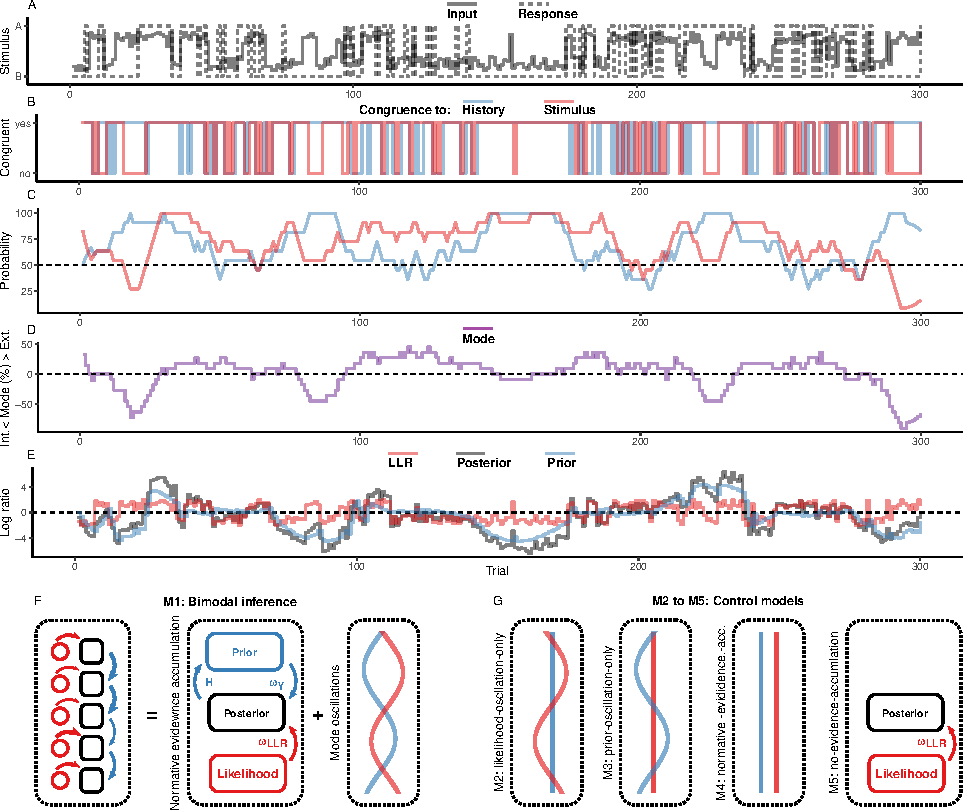
\includegraphics{modes_mouse_rev1b_clean_files/figure-latex/revised_Figure_1-1.pdf}

\textbf{Fig 1. Concept.}

A. In binary perceptual decision-making, a participant is presented with
stimuli from two categories (A vs.~B; dotted line) and reports
consecutive perceptual choices via button presses (sold line). All
panels below refer to these stimulated example data.

B. When the response matches the external stimulus information (i.e.,
overlap between dotted and solid line in panel A), perceptual choices
are \emph{stimulus-congruent} (red line). When the response matches the
response at the preceding trial, perceptual choices are
\emph{history-congruent} (blue line).

C. The dynamic probabilities of stimulus- and history-congruence (i.e.,
computed in sliding windows of ±5 trials) fluctuate over time.

D. The \emph{mode} of perceptual processing is derived by computing the
difference between the dynamic probabilities of stimulus- and
history-congruence. Values above 0\% indicate a bias toward external
information, whereas values below 0\% indicate a bias toward internal
information.

E. In computational modeling, internal mode is caused by an enhanced
impact of perceptual history. This causes the posterior (black line) to
be close to the prior (blue line). Conversely, during external mode, the
posterior is close to the sensory information (log likelihood ratio, red
line).

F. The bimodal inference model (M1) explains fluctuations between
externally- and externally-biased modes (left panel) by two interacting
factors: a normative accumulation of evidence according to parameters
\(H\) (middle panel), and anti-phase oscillations in the precision terms
\(\omega_{LLR}\) and \(\omega_{\psi}\) (right panel).

G. The control models M2-M5 were constructed by successively removing
the anti-phase oscillations and the integration of information from the
bimodal inference model. Please note that the
normative-evidence-accumulation-model (M4) corresponds to the model
proposed by Glaze et al.\textsuperscript{51}. In the
no-evidence-accumulation model (M5), perceptual decisions depend only on
likelihood information (flat priors).

\newpage

\hypertarget{figure-2}{%
\subsection{Figure 2}\label{figure-2}}

% 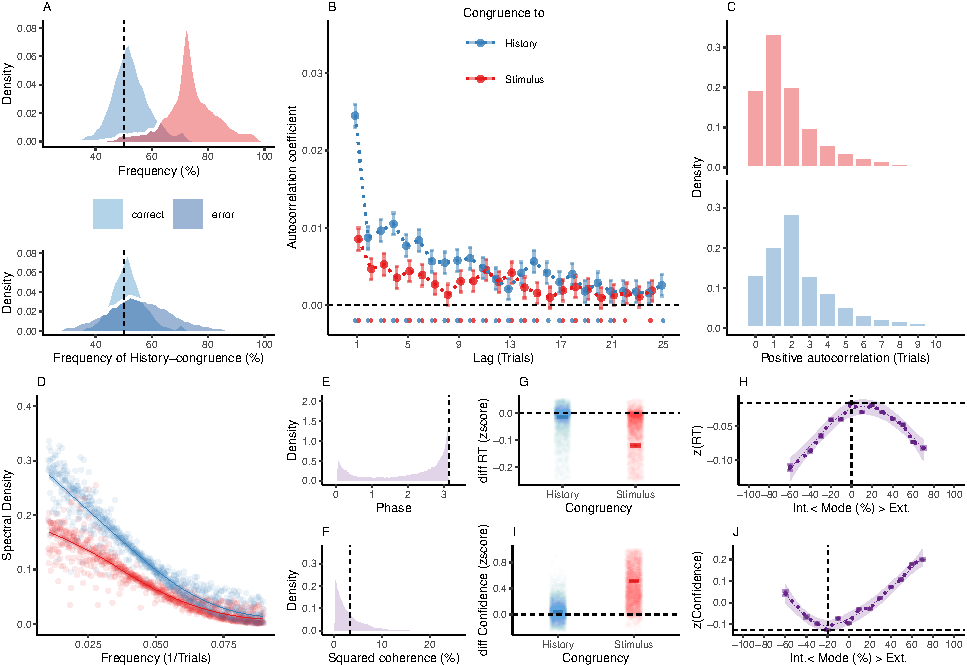
\includegraphics{modes_mouse_rev1b_clean_files/figure-latex/Figure_2-1.pdf}

\textbf{Fig 2. Internal and external modes in human perceptual
decision-making.}

A. In humans, perception was stimulus-congruent in 73.46\% ± 0.15\% (in
red) and history-congruent in 52.7\% ± 0.12\% of trials (in blue; upper
panel). History-congruent perceptual choices were more frequent when
perception was stimulus-incongruent (i.e., on \emph{error} trials; lower
panel), indicating that history effects impair performance in randomized
psychophysical designs.

B. Relative to randomly permuted data, we found highly significant
autocorrelations of stimulus-congruence and history-congruence (dots
indicate intercepts \(\neq\) 0 in trial-wise linear mixed effects
modeling at p \textless{} 0.05). Across trials, the autocorrelation
coefficients were best fit by an exponential function (adjusted \(R^2\)
for stimulus-congruence: 0.53; history-congruence: 0.72) as compared to
a linear function (adjusted \(R^2\) for stimulus-congruence: 0.53;
history-congruence: 0.51), decaying at a rate of \(\gamma\) =
\(\ensuremath{-1.92\times 10^{-3}}\) ±
\(\ensuremath{4.5\times 10^{-4}}\)
(T(\(\ensuremath{6.88\times 10^{4}}\)) = \(-4.27\), p =
\(\ensuremath{1.98\times 10^{-5}}\)) for stimulus-congruence and at a
rate of \(\gamma\) = \(\ensuremath{-6.11\times 10^{-3}}\) ±
\(\ensuremath{5.69\times 10^{-4}}\)
(T(\(\ensuremath{6.75\times 10^{4}}\)) = \(-10.74\), p =
\(\ensuremath{7.18\times 10^{-27}}\)) for history-congruence.

C. Here, we depict the number of consecutive trials at which
autocorrelation coefficients exceeded the respective autocorrelation of
randomly permuted data within individual participants. For
stimulus-congruence (upper panel), the lag of positive autocorrelation
amounted to \(3.24\) ± \(\ensuremath{2.39\times 10^{-3}}\) on average,
showing a peak at trial t+1 after the index trial. For
history-congruence (lower panel), the lag of positive autocorrelation
amounted to \(4.87\) ± \(\ensuremath{3.36\times 10^{-3}}\) on average,
peaking at trial t+2 after the index trial.

D. The smoothed probabilities of stimulus- and history-congruence
(sliding windows of ±5 trials) fluctuated as a scale-invariant process
with a 1/f power law, i.e., at power densities that were inversely
proportional to the frequency.

E. The distribution of phase shift between fluctuations in stimulus- and
history-congruence peaked at half a cycle (\(\pi\) denoted by dotted
line).

F. The average squared coherence between fluctuations in stimulus- and
history-congruence (black dotted line) amounted to \(6.49\) ±
\(\ensuremath{2.07\times 10^{-3}}\)\%

G. We observed faster RTs for both stimulus-congruence (as opposed to
stimulus-incongruence, \(\beta\) = \(-0.14\) ±
\(\ensuremath{1.6\times 10^{-3}}\),
T(\(\ensuremath{1.99\times 10^{6}}\)) = \(-85.84\), p < \(\ensuremath{2.2\times 10^{-308}}\)) and
history-congruence (\(\beta\) = \(\ensuremath{-9.56\times 10^{-3}}\) ±
\(\ensuremath{1.37\times 10^{-3}}\),
T(\(\ensuremath{1.98\times 10^{6}}\)) = \(-6.97\), p =
\(\ensuremath{3.15\times 10^{-12}}\)).

H. The mode of perceptual processing (i.e., the difference between the
smoothed probability of stimulus- vs.~history-congruence) showed a
quadratic relationship to RTs, with faster RTs for stronger biases
toward both external sensory information and internal predictions
provided by perceptual history (\(\beta_2\) = \(-19.86\) ± \(0.52\),
T(\(\ensuremath{1.98\times 10^{6}}\)) = \(-38.43\), p =
\(\ensuremath{5\times 10^{-323}}\)). The horizontal and vertical dotted
lines indicate maximum RT and the associated mode, respectively.

I. Confidence was enhanced for both stimulus-congruence (as opposed to
stimulus-incongruence, \(\beta\) = \(0.48\) ±
\(\ensuremath{1.38\times 10^{-3}}\),
T(\(\ensuremath{2.06\times 10^{6}}\)) = \(351.54\), p < \(\ensuremath{2.2\times 10^{-308}}\)) and
history-congruence (\(\beta\) = \(0.04\) ±
\(\ensuremath{1.18\times 10^{-3}}\),
T(\(\ensuremath{2.06\times 10^{6}}\)) = \(36.85\), p =
\(\ensuremath{3.25\times 10^{-297}}\)).

J. In analogy to RTs, we found a quadratic relationship between the mode
of perceptual processing and confidence, which increased when both
externally- and internally-biased modes grew stronger (\(\beta_2\) =
\(39.3\) ± \(0.94\), T(\(\ensuremath{2.06\times 10^{6}}\)) = \(41.95\),
p < \(\ensuremath{2.2\times 10^{-308}}\)). The horizontal and vertical dotted lines indicate minimum
confidence and the associated mode, respectively.

\newpage

\hypertarget{figure-3}{%
\subsection{Figure 3}\label{figure-3}}

% 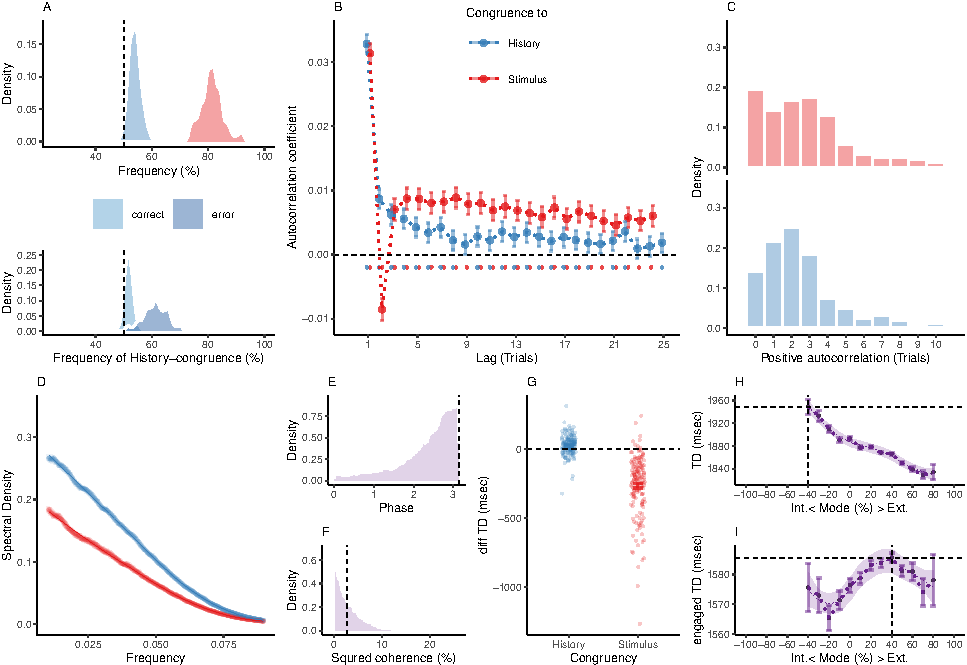
\includegraphics{modes_mouse_rev1b_clean_files/figure-latex/Figure_3-1.pdf}

\textbf{Fig 3. Internal and external modes in mouse perceptual
decision-making.}

A. In mice, 81.37\% ± 0.3\% of trials were stimulus-congruent (in red)
and 54.03\% ± 0.17\% of trials were history-congruent (in blue; upper
panel). History-congruent perceptual choices were not a consequence of
the experimental design, but a source of error, as they were more
frequent on stimulus-incongruent trials (lower panel).

B. Relative to randomly permuted data, we found highly significant
autocorrelations of stimulus-congruence and history-congruence (dots
indicate intercepts \(\neq\) 0 in trial-wise linear mixed effects
modeling at p \textless{} 0.05). Please note that the negative
autocorrelation of stimulus-congruence at trial 2 was a consequence of
the experimental design (S2 Fig). As in humans,
autocorrelation coefficients were best fit by an exponential function
(adjusted \(R^2\) for stimulus-congruence: \(0.44\); history-congruence:
\(0.52\)) as compared to a linear function (adjusted \(R^2\) for
stimulus-congruence: \(\ensuremath{3.16\times 10^{-3}}\);
history-congruence: \(0.26\)), decaying at a rate of \(\gamma\) =
\(\ensuremath{-6.2\times 10^{-4}}\) ±
\(\ensuremath{5.93\times 10^{-4}}\)
(T(\(\ensuremath{3.55\times 10^{4}}\)) = \(-1.05\), p = \(0.3\)) for
stimulus-congruence and at a rate of \(\gamma\) =
\(\ensuremath{-6.7\times 10^{-3}}\) ±
\(\ensuremath{5.94\times 10^{-4}}\)
(T(\(\ensuremath{3.69\times 10^{4}}\)) = \(-11.27\), p =
\(\ensuremath{2.07\times 10^{-29}}\)) for history-congruence.

C. For stimulus-congruence (upper panel), the lag of positive
autocorrelation was longer in comparison to humans (4.59 ± 0.06 on
average). For history-congruence (lower panel), the lag of positive
autocorrelation was slightly shorter relative to humans (2.58 ± 0.01 on
average, peaking at trial t+2 after the index trial).

D. In mice, the dynamic probabilities of stimulus- and
history-congruence (sliding windows of ±5 trials) fluctuated as a
scale-invariant process with a 1/f power law.

E. The distribution of phase shift between fluctuations in stimulus- and
history-congruence peaked at half a cycle (\(\pi\) denoted by dotted
line).

F. The average squared coherence between fluctuations in stimulus- and
history-congruence (black dotted line) amounted to 3.45 ± 0.01\%.

G. We observed shorter trial durations (TDs) for stimulus-congruence (as
opposed to stimulus-incongruence, \(\beta\) = \(-1.12\) ±
\(\ensuremath{8.53\times 10^{-3}}\),
T(\(\ensuremath{1.34\times 10^{6}}\)) = \(-131.78\), p < \(\ensuremath{2.2\times 10^{-308}}\)), but
longer TDs for history-congruence (\(\beta\) = \(0.06\) ±
\(\ensuremath{6.76\times 10^{-3}}\),
T(\(\ensuremath{1.34\times 10^{6}}\)) = \(8.52\), p =
\(\ensuremath{1.58\times 10^{-17}}\)).

H. TDs decreased monotonically for stronger biases toward external mode
(\(\beta_1\) = \(\ensuremath{-4.16\times 10^{4}}\) ±
\(\ensuremath{1.29\times 10^{3}}\),
T(\(\ensuremath{1.35\times 10^{6}}\)) = \(-32.31\), p =
\(\ensuremath{6.03\times 10^{-229}}\)). The horizontal and vertical
dotted lines indicate maximum TD and the associated mode, respectively.

I. For TDs that differed from the median TD by no more than 1.5 x MAD
(median absolute distance\textsuperscript{49}), mice exhibited a
quadratic component in the relationship between the mode of sensory
processing and TDs (\(\beta_2\) = \(\ensuremath{-1.97\times 10^{3}}\) ±
\(843.74\), T(\(\ensuremath{1.19\times 10^{6}}\)) = \(-2.34\), p =
\(0.02\)). This explorative post-hoc analysis focuses on trials at which
mice engage more swiftly with the experimental task. The horizontal and
vertical dotted lines indicate maximum TD and the associated mode,
respectively.

\newpage

\hypertarget{figure-4}{%
\subsection{Figure 4}\label{figure-4}}

% 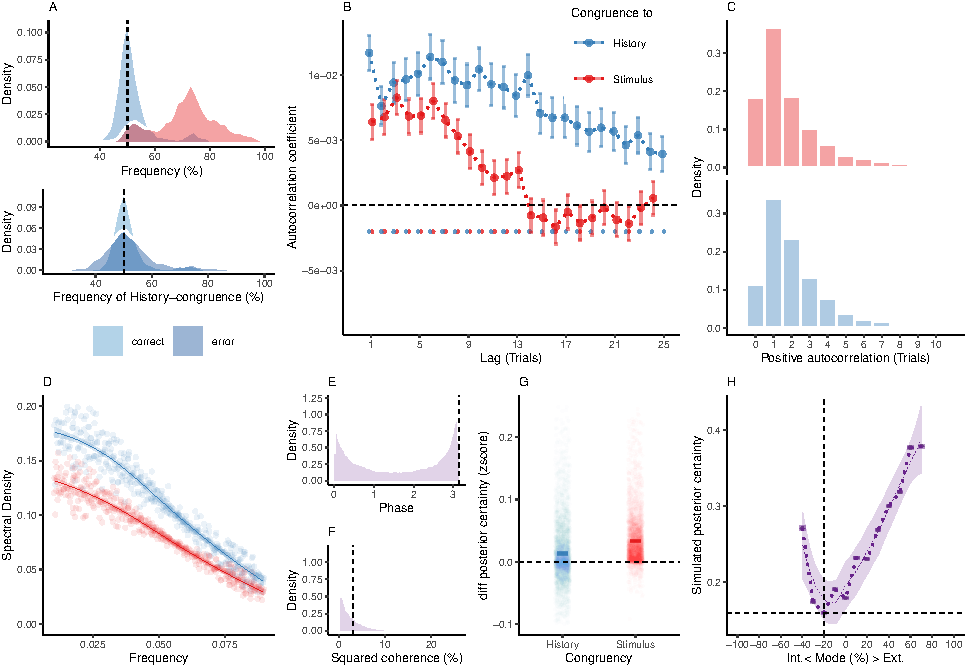
\includegraphics{modes_mouse_rev1b_clean_files/figure-latex/Figure_4-1.pdf}

\textbf{Fig 4. Internal and external modes in simulated perceptual
decision-making.}

A. Simulated perceptual choices were stimulus-congruent in 71.36\% ±
0.17\% (in red) and history-congruent in 51.99\% ± 0.11\% of trials (in
blue; T(\(\ensuremath{4.32\times 10^{3}}\)) = \(17.42\), p =
\(\ensuremath{9.89\times 10^{-66}}\); upper panel). Due to the
competition between stimulus- and history-congruence, history-congruent
perceptual choices were more frequent when perception was
stimulus-incongruent (i.e., on \emph{error} trials;
T(\ensuremath{4.32\times 10^{3}}) = 11.19, p =
\(\ensuremath{1.17\times 10^{-28}}\); lower panel) and thus impaired
performance in the randomized psychophysical design simulated here.

B. At the simulated group level, we found significant autocorrelations
in both stimulus-congruence (13 consecutive trials) and
history-congruence (30 consecutive trials).

C. On the level of individual simulated participants, autocorrelation
coefficients exceeded the autocorrelation coefficients of randomly
permuted data within a lag of \(2.46\) ±
\(\ensuremath{1.17\times 10^{-3}}\) trials for stimulus-congruence and
\(4.24\) ± \(\ensuremath{1.85\times 10^{-3}}\) trials for
history-congruence.

D. The smoothed probabilities of stimulus- and history-congruence
(sliding windows of ±5 trials) fluctuated as a scale-invariant process
with a 1/f power law, i.e., at power densities that were inversely
proportional to the frequency (power \textasciitilde{} 1/\(f^\beta\);
stimulus-congruence: \(\beta\) = \(-0.81\) ±
\(\ensuremath{1.18\times 10^{-3}}\),
T(\(\ensuremath{1.92\times 10^{5}}\)) = \(-687.58\), p < \(\ensuremath{2.2\times 10^{-308}}\);
history-congruence: \(\beta\) = \(-0.83\) ±
\(\ensuremath{1.27\times 10^{-3}}\),
T(\(\ensuremath{1.92\times 10^{5}}\)) = \(-652.11\), p < \(\ensuremath{2.2\times 10^{-308}}\)).

E. The distribution of phase shift between fluctuations in simulated
stimulus- and history-congruence peaked at half a cycle (\(\pi\) denoted
by dotted line). The dynamic probabilities of simulated stimulus- and
history-congruence were therefore were strongly anti-correlated
(\(\beta\) = \(-0.03\) ± \(\ensuremath{8.22\times 10^{-4}}\),
T(\(\ensuremath{2.12\times 10^{6}}\)) = \(-40.52\), p < \(\ensuremath{2.2\times 10^{-308}}\)).

F. The average squared coherence between fluctuations in simulated
stimulus- and history-congruence (black dotted line) amounted to
\(6.49\) ± \(\ensuremath{2.07\times 10^{-3}}\)\%.

G. Simulated confidence was enhanced for stimulus-congruence (\(\beta\)
= \(0.03\) ± \(\ensuremath{1.71\times 10^{-4}}\),
T(\(\ensuremath{2.03\times 10^{6}}\)) = \(178.39\), p < \(\ensuremath{2.2\times 10^{-308}}\)) and
history-congruence (\(\beta\) = \(0.01\) ±
\(\ensuremath{1.5\times 10^{-4}}\),
T(\(\ensuremath{2.03\times 10^{6}}\)) = \(74.18\), p < \(\ensuremath{2.2\times 10^{-308}}\)).

H. In analogy to humans, the simulated data showed a quadratic
relationship between the mode of perceptual processing and posterior
certainty, which increased for stronger external and internal biases
(\(\beta_2\) = \(31.03\) ± \(0.15\),
T(\(\ensuremath{2.04\times 10^{6}}\)) = \(205.95\), p < \(\ensuremath{2.2\times 10^{-308}}\)). The
horizontal and vertical dotted lines indicate minimum posterior
certainty and the associated mode, respectively.

\newpage
\hypertarget{references}{%
\section*{References}\label{references}}
\addcontentsline{toc}{section}{References}

\hypertarget{refs}{}
\begin{CSLReferences}{0}{0}
\leavevmode\vadjust pre{\hypertarget{ref-Schrodinger1944}{}}%
\CSLLeftMargin{1. }%
\CSLRightInline{Schrödinger, E.
\emph{\href{http://filf.pskgu.ru/ebooks/schbio/schbio_titul.pdf}{What is
life? The physical aspect of the living cell}}. (Cambridge University
Press, 1944).}

\leavevmode\vadjust pre{\hypertarget{ref-Ashby1947}{}}%
\CSLLeftMargin{2. }%
\CSLRightInline{Ashby, W. R.
\href{https://doi.org/10.1080/00221309.1947.9918144}{Principles of the
self-organizing dynamic system}. \emph{Journal of General Psychology}
\textbf{37}, 125--128 (1947).}

\leavevmode\vadjust pre{\hypertarget{ref-Friston2013}{}}%
\CSLLeftMargin{3. }%
\CSLRightInline{Friston, K. \emph{et al.}
\href{https://doi.org/10.3389/fnhum.2013.00598}{The anatomy of choice:
Active inference and agency.} \emph{Frontiers in human neuroscience}
\textbf{7}, 598 (2013).}

\leavevmode\vadjust pre{\hypertarget{ref-Palva2011}{}}%
\CSLLeftMargin{4. }%
\CSLRightInline{Palva, J. M. \emph{et al.}
\href{https://doi.org/10.1016/B978-0-444-53839-0.00022-3}{Roles of
multiscale brain activity fluctuations in shaping the variability and
dynamics of psychophysical performance}. in \emph{Progress in Brain
Research} vol. 193 335--350 (Elsevier B.V., 2011).}

\leavevmode\vadjust pre{\hypertarget{ref-VanRullen2016}{}}%
\CSLLeftMargin{5. }%
\CSLRightInline{VanRullen, R.
\href{https://doi.org/10.1016/j.tics.2016.07.006}{Perceptual cycles}.
\emph{Trends in Cognitive Sciences} \textbf{20}, 723--735 (2016).}

\leavevmode\vadjust pre{\hypertarget{ref-Verplanck1952}{}}%
\CSLLeftMargin{6. }%
\CSLRightInline{Verplanck, W. \emph{et al.}
\href{https://psycnet.apa.org/record/1953-04864-001}{Nonindependence of
successive responses in measurements of the visual threshold.}
\emph{psycnet.apa.org} (1952).}

\leavevmode\vadjust pre{\hypertarget{ref-Atkinson1963}{}}%
\CSLLeftMargin{7. }%
\CSLRightInline{Atkinson, R. C.
\href{https://doi.org/10.1037/h0041428}{A variable sensitivity theory of
signal detection}. \emph{Psychological Review} \textbf{70}, 91--106
(1963).}

\leavevmode\vadjust pre{\hypertarget{ref-Dehaene1993}{}}%
\CSLLeftMargin{8. }%
\CSLRightInline{Dehaene, S.
\href{https://doi.org/10.1111/j.1467-9280.1993.tb00273.x}{Temporal
oscillations in human perception}. \emph{Psychological Science}
\textbf{4}, 264--270 (1993).}

\leavevmode\vadjust pre{\hypertarget{ref-Gilden1995}{}}%
\CSLLeftMargin{9. }%
\CSLRightInline{Gilden, D. L. \emph{et al.}
\href{https://doi.org/10.1006/cogp.1995.1002}{On the nature of streaks
in signal detection}. \emph{Cognitive Psychology} \textbf{28}, 17--64
(1995).}

\leavevmode\vadjust pre{\hypertarget{ref-Gilden1995a}{}}%
\CSLLeftMargin{10. }%
\CSLRightInline{Gilden, D. L. \emph{et al.}
\href{https://doi.org/10.1126/science.7892611}{1/f noise in human
cognition}. \emph{Science} \textbf{67}, 1837--1839 (1995).}

\leavevmode\vadjust pre{\hypertarget{ref-Monto2008}{}}%
\CSLLeftMargin{11. }%
\CSLRightInline{Monto, S. \emph{et al.}
\href{https://doi.org/10.1523/JNEUROSCI.1910-08.2008}{Very slow EEG
fluctuations predict the dynamics of stimulus detection and oscillation
amplitudes in humans}. \emph{Journal of Neuroscience} \textbf{28},
8268--8272 (2008).}

\leavevmode\vadjust pre{\hypertarget{ref-Ashwood2022}{}}%
\CSLLeftMargin{12. }%
\CSLRightInline{Ashwood, Z. C. \emph{et al.}
\href{https://doi.org/10.1038/s41593-021-01007-z}{Mice alternate between
discrete strategies during perceptual decision-making}. \emph{Nature
Neuroscience} \textbf{25}, 201--212 (2022).}

\leavevmode\vadjust pre{\hypertarget{ref-Gilden2001}{}}%
\CSLLeftMargin{13. }%
\CSLRightInline{Gilden, D. L.
\href{https://doi.org/10.1037/0033-295X.108.1.33}{Cognitive emissions of
1/f noise}. \emph{Psychological Review} \textbf{108}, 33--56 (2001).}

\leavevmode\vadjust pre{\hypertarget{ref-Duncan2012}{}}%
\CSLLeftMargin{14. }%
\CSLRightInline{Duncan, K. \emph{et al.}
\href{https://doi.org/10.1126/science.1221936}{Memory's penumbra:
Episodic memory decisions induce lingering mnemonic biases}.
\emph{Science} \textbf{337}, 485--487 (2012).}

\leavevmode\vadjust pre{\hypertarget{ref-ClareKelly2008}{}}%
\CSLLeftMargin{15. }%
\CSLRightInline{Kelly, A. M. C. \emph{et al.}
\href{https://doi.org/10.1016/j.neuroimage.2007.08.008}{Competition
between functional brain networks mediates behavioral variability}.
\emph{NeuroImage} \textbf{39}, 527--537 (2008).}

\leavevmode\vadjust pre{\hypertarget{ref-Hesselmann2008}{}}%
\CSLLeftMargin{16. }%
\CSLRightInline{Hesselmann, G. \emph{et al.}
\href{https://doi.org/10.1073/pnas.0712043105}{Spontaneous local
variations in ongoing neural activity bias perceptual decisions}.
\emph{Proceedings of the National Academy of Sciences of the United
States of America} \textbf{105}, 10984--10989 (2008).}

\leavevmode\vadjust pre{\hypertarget{ref-Schroeder2010a}{}}%
\CSLLeftMargin{17. }%
\CSLRightInline{Schroeder, C. E. \emph{et al.}
\href{https://doi.org/10.1016/j.conb.2010.02.010}{Dynamics of active
sensing and perceptual selection}. \emph{Current Opinion in
Neurobiology} \textbf{20}, 172--176 (2010).}

\leavevmode\vadjust pre{\hypertarget{ref-Honey2017}{}}%
\CSLLeftMargin{18. }%
\CSLRightInline{Honey, C. J. \emph{et al.}
\href{https://doi.org/10.1162/netn_a_00024}{Switching between internal
and external modes: A multiscale learning principle}. \emph{Network
Neuroscience} \textbf{1}, 339--356 (2017).}

\leavevmode\vadjust pre{\hypertarget{ref-Weilnhammer2021a}{}}%
\CSLLeftMargin{19. }%
\CSLRightInline{Weilnhammer, V. \emph{et al.}
\href{https://doi.org/10.1016/j.isci.2021.102234}{Bistable perception
alternates between internal and external modes of sensory processing}.
\emph{iScience} \textbf{24}, (2021).}

\leavevmode\vadjust pre{\hypertarget{ref-Rahnev2020}{}}%
\CSLLeftMargin{20. }%
\CSLRightInline{Rahnev, D. \emph{et al.}
\href{https://doi.org/10.1038/s41562-019-0813-1}{The confidence
database}. \emph{Nature Human Behaviour} \textbf{4}, 317--325 (2020).}h

\leavevmode\vadjust pre{\hypertarget{ref-IBL2021}{}}%
\CSLLeftMargin{21. }%
\CSLRightInline{Aguillon-Rodriguez, V. \emph{et al.}
\href{https://doi.org/10.7554/ELIFE.63711}{Standardized and reproducible
measurement of decision-making in mice}. \emph{eLife} \textbf{10},
(2021).}

\leavevmode\vadjust pre{\hypertarget{ref-fischer_serial_2014}{}}%
\CSLLeftMargin{22. }%
\CSLRightInline{Fischer, J. \emph{et al.}
\href{https://doi.org/10.1038/nn.3689}{Serial dependence in visual
perception}. \emph{Nat. Neurosci.} \textbf{17}, 738--743 (2014).}

\leavevmode\vadjust pre{\hypertarget{ref-Liberman2014}{}}%
\CSLLeftMargin{23. }%
\CSLRightInline{Liberman, A. \emph{et al.}
\href{https://doi.org/10.1016/j.cub.2014.09.025}{Serial dependence in
the perception of faces}. \emph{Current Biology} \textbf{24}, 2569--2574
(2014).}

\leavevmode\vadjust pre{\hypertarget{ref-Abrahamyan2016}{}}%
\CSLLeftMargin{24. }%
\CSLRightInline{Abrahamyan, A. \emph{et al.}
\href{https://doi.org/10.1073/pnas.1518786113}{Adaptable history biases
in human perceptual decisions}. \emph{Proceedings of the National
Academy of Sciences of the United States of America} \textbf{113},
E3548--E3557 (2016).}

\leavevmode\vadjust pre{\hypertarget{ref-Cicchini2014}{}}%
\CSLLeftMargin{25. }%
\CSLRightInline{Cicchini, G. M. \emph{et al.}
\href{https://doi.org/10.1073/pnas.1402785111}{Compressive mapping of
number to space reflects dynamic encoding mechanisms, not static
logarithmic transform}. \emph{Proceedings of the National Academy of
Sciences of the United States of America} \textbf{111}, 7867--7872
(2014).}

\leavevmode\vadjust pre{\hypertarget{ref-Cicchini2017}{}}%
\CSLLeftMargin{26. }%
\CSLRightInline{Cicchini, G. M. \emph{et al.}
\href{https://doi.org/10.1167/17.14.6}{Serial dependencies act directly
on perception}. \emph{Journal of Vision} \textbf{17}, (2017).}

\leavevmode\vadjust pre{\hypertarget{ref-Fritsche2020}{}}%
\CSLLeftMargin{27. }%
\CSLRightInline{Fritsche, M. \emph{et al.}
\href{https://doi.org/10.7554/eLife.55389}{A bayesian and efficient
observer model explains concurrent attractive and repulsive history
biases in visual perception}. \emph{eLife} \textbf{9}, 1--32 (2020).}

\leavevmode\vadjust pre{\hypertarget{ref-Urai2017}{}}%
\CSLLeftMargin{28. }%
\CSLRightInline{Urai, A. E. \emph{et al.}
\href{https://doi.org/10.1038/ncomms14637}{Pupil-linked arousal is
driven by decision uncertainty and alters serial choice bias}.
\emph{Nature Communications} \textbf{8}, (2017).}

\leavevmode\vadjust pre{\hypertarget{ref-Akrami2018}{}}%
\CSLLeftMargin{29. }%
\CSLRightInline{Akrami, A. \emph{et al.}
\href{https://doi.org/10.1038/nature25510}{Posterior parietal cortex
represents sensory history and mediates its effects on behaviour}.
\emph{Nature} \textbf{554}, 368--372 (2018).}

\leavevmode\vadjust pre{\hypertarget{ref-Braun2018}{}}%
\CSLLeftMargin{30. }%
\CSLRightInline{Braun, A. \emph{et al.}
\href{https://doi.org/10.1523/JNEUROSCI.2189-17.2017}{Adaptive history
biases result from confidence-weighted accumulation of past choices}.
\emph{Journal of Neuroscience} \textbf{38}, 2418--2429 (2018).}

\leavevmode\vadjust pre{\hypertarget{ref-Bergen2019}{}}%
\CSLLeftMargin{31. }%
\CSLRightInline{Bergen, R. S. V. \emph{et al.}
\href{https://doi.org/10.1523/JNEUROSCI.3212-18.2019}{Probabilistic
representation in human visual cortex reflects uncertainty in serial
decisions}. \emph{Journal of Neuroscience} \textbf{39}, 8164--8176
(2019).}

\leavevmode\vadjust pre{\hypertarget{ref-Urai2019}{}}%
\CSLLeftMargin{32. }%
\CSLRightInline{Urai, A. E. \emph{et al.}
\href{https://doi.org/10.7554/eLife.46331}{Choice history biases
subsequent evidence accumulation}. \emph{eLife} \textbf{8}, (2019).}

\leavevmode\vadjust pre{\hypertarget{ref-Hsu2020}{}}%
\CSLLeftMargin{33. }%
\CSLRightInline{Hsu, S. M. \emph{et al.}
\href{https://doi.org/10.1080/02699931.2019.1696752}{The roles of
preceding stimuli and preceding responses on assimilative and
contrastive sequential effects during facial expression perception}.
\emph{Cognition and Emotion} \textbf{34}, 890--905 (2020).}

\leavevmode\vadjust pre{\hypertarget{ref-Dong1995}{}}%
\CSLLeftMargin{34. }%
\CSLRightInline{Dong, D. W. \emph{et al.}
\href{https://doi.org/10.1088/0954-898X_6_3_003}{Statistics of natural
time-varying images}. \emph{Network: Computation in Neural Systems}
\textbf{6}, 345--358 (1995).}

\leavevmode\vadjust pre{\hypertarget{ref-Burr2014}{}}%
\CSLLeftMargin{35. }%
\CSLRightInline{Burr, D. \emph{et al.}
\href{https://doi.org/10.1016/j.cub.2014.10.002}{Vision: Efficient
adaptive coding}. \emph{Current Biology} vol. 24 R1096--R1098 (2014).}

\leavevmode\vadjust pre{\hypertarget{ref-Montroll1982}{}}%
\CSLLeftMargin{36. }%
\CSLRightInline{Montroll, E. W. \emph{et al.}
\href{https://doi.org/10.1073/pnas.79.10.3380}{On 1/f noise and other
distributions with long tails}. \emph{Proceedings of the National
Academy of Sciences} \textbf{79}, 3380--3383 (1982).}

\leavevmode\vadjust pre{\hypertarget{ref-Bak1987}{}}%
\CSLLeftMargin{37. }%
\CSLRightInline{Bak, P. \emph{et al.}
\href{https://doi.org/10.1103/PhysRevLett.59.381}{Self-organized
criticality: An explanation of the 1/f noise}. \emph{Physical Review
Letters} \textbf{59}, 381--384 (1987).}

\leavevmode\vadjust pre{\hypertarget{ref-Chialvo2010}{}}%
\CSLLeftMargin{38. }%
\CSLRightInline{Chialvo, D. R.
\href{https://doi.org/10.1038/nphys1803}{Emergent complex neural
dynamics}. \emph{Nature Physics} \textbf{6}, 744--750 (2010).}

\leavevmode\vadjust pre{\hypertarget{ref-Wagenmakers2004}{}}%
\CSLLeftMargin{39. }%
\CSLRightInline{Wagenmakers, E. J. \emph{et al.}
\href{https://doi.org/10.3758/BF03196615}{Estimation and interpretation
of 1/f noise in human cognition}. \emph{Psychonomic Bulletin and Review}
\textbf{11}, 579--615 (2004).}

\leavevmode\vadjust pre{\hypertarget{ref-VanOrden2005}{}}%
\CSLLeftMargin{40. }%
\CSLRightInline{Orden, G. C. V. \emph{et al.}
\href{https://doi.org/10.1037/0096-3445.134.1.117}{Human cognition and
1/f scaling}. \emph{Journal of Experimental Psychology: General}
\textbf{134}, 117--123 (2005).}

\leavevmode\vadjust pre{\hypertarget{ref-Chopin2012}{}}%
\CSLLeftMargin{41. }%
\CSLRightInline{Chopin, A. \emph{et al.}
\href{https://doi.org/10.1016/j.cub.2012.02.021}{Predictive properties
of visual adaptation}. \emph{Current Biology} \textbf{22}, 622--626
(2012).}

\leavevmode\vadjust pre{\hypertarget{ref-Cicchini2018}{}}%
\CSLLeftMargin{42. }%
\CSLRightInline{Cicchini, G. M. \emph{et al.}
\href{https://doi.org/10.1098/rspb.2018.1722}{The functional role of
serial dependence}. \emph{Proceedings of the Royal Society B: Biological
Sciences} \textbf{285}, (2018).}

\leavevmode\vadjust pre{\hypertarget{ref-Kiyonaga2017}{}}%
\CSLLeftMargin{43. }%
\CSLRightInline{Kiyonaga, A. \emph{et al.}
\href{https://doi.org/10.1016/j.tics.2017.04.011}{Serial dependence
across perception, attention, and memory}. \emph{Trends in Cognitive
Sciences} \textbf{21}, 493--497 (2017).}

\leavevmode\vadjust pre{\hypertarget{ref-Kepecs2008}{}}%
\CSLLeftMargin{44. }%
\CSLRightInline{Kepecs, A. \emph{et al.}
\href{https://doi.org/10.1038/nature07200}{Neural correlates,
computation and behavioural impact of decision confidence}.
\emph{Nature} \textbf{455}, 227--231 (2008).}

\leavevmode\vadjust pre{\hypertarget{ref-Fleming2014}{}}%
\CSLLeftMargin{45. }%
\CSLRightInline{Fleming, S. M. \emph{et al.}
\href{https://doi.org/10.3389/fnhum.2014.00443}{How to measure
metacognition}. \emph{Frontiers in Human Neuroscience} \textbf{8}, 443
(2014).}

\leavevmode\vadjust pre{\hypertarget{ref-St.John-Saaltink2016}{}}%
\CSLLeftMargin{46. }%
\CSLRightInline{John-Saaltink, E. St. \emph{et al.}
\href{https://doi.org/10.1523/JNEUROSCI.4390-15.2016}{Serial dependence
in perceptual decisions is reflected in activity patterns in primary
visual cortex}. \emph{Journal of Neuroscience} \textbf{36}, 6186--6192
(2016).}

\leavevmode\vadjust pre{\hypertarget{ref-Cicchini2021}{}}%
\CSLLeftMargin{47. }%
\CSLRightInline{Cicchini, G. M. \emph{et al.}
\href{https://doi.org/10.1016/j.cub.2020.12.004}{Perceptual history
propagates down to early levels of sensory analysis}. \emph{Current
Biology} \textbf{31}, 1245--1250.e2 (2021).}

\leavevmode\vadjust pre{\hypertarget{ref-Akaike1987}{}}%
\CSLLeftMargin{48. }%
\CSLRightInline{Akaike, H.
\href{https://doi.org/10.1007/BF02294359}{Factor analysis and AIC}.
\emph{Psychometrika} \textbf{52}, 317--332 (1987).}

\leavevmode\vadjust pre{\hypertarget{ref-Leys2013}{}}%
\CSLLeftMargin{49. }%
\CSLRightInline{Leys, C. \emph{et al.}
\href{https://doi.org/10.1016/J.JESP.2013.03.013}{Detecting outliers: Do
not use standard deviation around the mean, use absolute deviation
around the median}. \emph{Journal of Experimental Social Psychology}
\textbf{49}, 764--766 (2013).}

\leavevmode\vadjust pre{\hypertarget{ref-Maloney2005}{}}%
\CSLLeftMargin{50. }%
\CSLRightInline{Maloney, L. T. \emph{et al.}
\href{https://doi.org/10.1073/pnas.0407157102}{Past trials influence
perception of ambiguous motion quartets through pattern completion}.
\emph{Proceedings of the National Academy of Sciences of the United
States of America} \textbf{102}, 3164--3169 (2005).}

\leavevmode\vadjust pre{\hypertarget{ref-Glaze2015}{}}%
\CSLLeftMargin{51. }%
\CSLRightInline{Glaze, C. M. \emph{et al.}
\href{https://doi.org/10.7554/eLife.08825}{Normative evidence
accumulation in unpredictable environments}. \emph{eLife} \textbf{4},
(2015).}

\leavevmode\vadjust pre{\hypertarget{ref-Wexler2015}{}}%
\CSLLeftMargin{52. }%
\CSLRightInline{Wexler, M. \emph{et al.}
\href{https://doi.org/10.1073/pnas.1508847112}{Persistent states in
vision break universality and time invariance}. \emph{Proceedings of the
National Academy of Sciences of the United States of America}
\textbf{112}, 14990--14995 (2015).}

\leavevmode\vadjust pre{\hypertarget{ref-Feldman2010}{}}%
\CSLLeftMargin{53. }%
\CSLRightInline{Feldman, H. \emph{et al.}
\href{https://doi.org/10.3389/FNHUM.2010.00215/BIBTEX}{Attention,
uncertainty, and free-energy}. \emph{Frontiers in Human Neuroscience}
\textbf{4}, 7028 (2010).}

\leavevmode\vadjust pre{\hypertarget{ref-Mathys2014a}{}}%
\CSLLeftMargin{54. }%
\CSLRightInline{Mathys, C. D. \emph{et al.}
\href{https://doi.org/10.3389/fnhum.2014.00825}{Uncertainty in
perception and the hierarchical gaussian filter.} \emph{Frontiers in
human neuroscience} \textbf{8}, 825 (2014).}

\leavevmode\vadjust pre{\hypertarget{ref-Friston2005}{}}%
\CSLLeftMargin{55. }%
\CSLRightInline{Friston, K.
\href{https://doi.org/10.1098/rstb.2005.1622}{A theory of cortical
responses.} \emph{Philosophical transactions of the Royal Society of
London. Series B, Biological sciences} \textbf{360}, 815--836 (2005).}

\leavevmode\vadjust pre{\hypertarget{ref-Sterzer2018}{}}%
\CSLLeftMargin{56. }%
\CSLRightInline{Sterzer, P. \emph{et al.}
\href{https://doi.org/10.1016/j.biopsych.2018.05.015}{The predictive
coding account of psychosis}. \emph{Biological Psychiatry} \textbf{84},
634--643 (2018).}

\leavevmode\vadjust pre{\hypertarget{ref-Jardri2017}{}}%
\CSLLeftMargin{57. }%
\CSLRightInline{Jardri, R. \emph{et al.}
\href{https://doi.org/10.1038/ncomms14218}{Experimental evidence for
circular inference in schizophrenia}. \emph{Nature Communications}
\textbf{8}, 14218 (2017).}

\leavevmode\vadjust pre{\hypertarget{ref-Bengio2015}{}}%
\CSLLeftMargin{58. }%
\CSLRightInline{Bengio, Y. \emph{et al.}
\href{http://arxiv.org/abs/1502.04156}{Towards biologically plausible
deep learning}. \emph{bioRxiv} (2015).}

\leavevmode\vadjust pre{\hypertarget{ref-Dijkstra2021}{}}%
\CSLLeftMargin{59. }%
\CSLRightInline{Dijkstra, N. \emph{et al.} Perceptual reality
monitoring: Neural mechanisms dissociating imagination from reality.
\emph{PsyArXiv} (2021)
doi:\href{https://doi.org/10.31234/OSF.IO/ZNGEQ}{10.31234/OSF.IO/ZNGEQ}.}

\leavevmode\vadjust pre{\hypertarget{ref-Bitzer2014}{}}%
\CSLLeftMargin{60. }%
\CSLRightInline{Bitzer, S. \emph{et al.}
\href{https://doi.org/10.3389/FNHUM.2014.00102/BIBTEX}{Perceptual
decision making: Drift-diffusion model is equivalent to a bayesian
model}. \emph{Frontiers in Human Neuroscience} \textbf{8}, 77624
(2014).}

\leavevmode\vadjust pre{\hypertarget{ref-Roy2021}{}}%
\CSLLeftMargin{61. }%
\CSLRightInline{Roy, N. A. \emph{et al.}
\href{https://doi.org/10.1016/J.NEURON.2020.12.004}{Extracting the
dynamics of behavior in sensory decision-making experiments}.
\emph{Neuron} \textbf{109}, 597--610.e6 (2021).}

\leavevmode\vadjust pre{\hypertarget{ref-Ashwood2021}{}}%
\CSLLeftMargin{62. }%
\CSLRightInline{Ashwood, Z. C. \emph{et al.} Mice alternate between
discrete strategies during perceptual decision-making. \emph{bioRxiv}
2020.10.19.346353 (2021)
doi:\href{https://doi.org/10.1101/2020.10.19.346353}{10.1101/2020.10.19.346353}.}

\leavevmode\vadjust pre{\hypertarget{ref-Matthews2010}{}}%
\CSLLeftMargin{63. }%
\CSLRightInline{Matthews, G. \emph{et al.} Task engagement, attention,
and executive control. 205--230 (2010)
doi:\href{https://doi.org/10.1007/978-1-4419-1210-7_13}{10.1007/978-1-4419-1210-7\_13}.}

\leavevmode\vadjust pre{\hypertarget{ref-McGinley2015}{}}%
\CSLLeftMargin{64. }%
\CSLRightInline{McGinley, M. J. \emph{et al.}
\href{https://doi.org/10.1016/j.neuron.2015.09.012}{Waking state: Rapid
variations modulate neural and behavioral responses}. \emph{Neuron}
\textbf{87}, 1143--1161 (2015).}

\leavevmode\vadjust pre{\hypertarget{ref-Beerendonk2023}{}}%
\CSLLeftMargin{65. }%
\CSLRightInline{Beerendonk, L. \emph{et al.} A disinhibitory circuit
mechanism explains a general principle of peak performance during
mid-level arousal. \emph{bioRxiv} 2023.07.28.550956 (2023)
doi:\href{https://doi.org/10.1101/2023.07.28.550956}{10.1101/2023.07.28.550956}.}

\leavevmode\vadjust pre{\hypertarget{ref-Gee2014}{}}%
\CSLLeftMargin{66. }%
\CSLRightInline{Gee, J. W. D. \emph{et al.}
\href{https://doi.org/10.1073/PNAS.1317557111/SUPPL_FILE/PNAS.201317557SI.PDF}{Decision-related
pupil dilation reflects upcoming choice and individual bias}.
\emph{Proceedings of the National Academy of Sciences of the United
States of America} \textbf{111}, E618--E625 (2014).}

\leavevmode\vadjust pre{\hypertarget{ref-Gee2017}{}}%
\CSLLeftMargin{67. }%
\CSLRightInline{Gee, J. W. de \emph{et al.}
\href{https://doi.org/10.7554/ELIFE.23232}{Dynamic modulation of
decision biases by brainstem arousal systems}. \emph{eLife} \textbf{6},
(2017).}

\leavevmode\vadjust pre{\hypertarget{ref-Gee2020}{}}%
\CSLLeftMargin{68. }%
\CSLRightInline{Gee, J. W. de \emph{et al.}
\href{https://doi.org/10.7554/ELIFE.54014}{Pupil-linked phasic arousal
predicts a reduction of choice bias across species and decision
domains}. \emph{eLife} \textbf{9}, 1--25 (2020).}

\leavevmode\vadjust pre{\hypertarget{ref-McGinley2015b}{}}%
\CSLLeftMargin{69. }%
\CSLRightInline{McGinley, M. J. \emph{et al.}
\href{https://doi.org/10.1016/j.neuron.2015.09.012}{Waking state: Rapid
variations modulate neural and behavioral responses}. \emph{Neuron}
\textbf{87}, 1143--1161 (2015).}

\leavevmode\vadjust pre{\hypertarget{ref-Gee2022}{}}%
\CSLLeftMargin{70. }%
\CSLRightInline{Gee, J. W. de \emph{et al.} Mice regulate their
attentional intensity and arousal to exploit increases in task utility.
\emph{bioRxiv} 2022.03.04.482962 (2022)
doi:\href{https://doi.org/10.1101/2022.03.04.482962}{10.1101/2022.03.04.482962}.}

\leavevmode\vadjust pre{\hypertarget{ref-IBL2023}{}}%
\CSLLeftMargin{71. }%
\CSLRightInline{Laboratory, I. B. \emph{et al.} A brain-wide map of
neural activity during complex behaviour.
doi:\href{https://doi.org/10.1101/2023.07.04.547681}{10.1101/2023.07.04.547681}.}

\leavevmode\vadjust pre{\hypertarget{ref-Mawase2018}{}}%
\CSLLeftMargin{72. }%
\CSLRightInline{Mawase, F. \emph{et al.}
\href{https://doi.org/10.1016/J.CELREP.2018.06.097}{Movement repetition
facilitates response preparation}. \emph{Cell reports} \textbf{24},
801--808 (2018).}

\leavevmode\vadjust pre{\hypertarget{ref-Pomper2023}{}}%
\CSLLeftMargin{73. }%
\CSLRightInline{Pomper, U. \emph{et al.}
\href{https://doi.org/10.1111/PSYP.14172}{Motor-induced oscillations in
choice response performance}. \emph{Psychophysiology} \textbf{60},
e14172 (2023).}

\leavevmode\vadjust pre{\hypertarget{ref-Kepecs2012}{}}%
\CSLLeftMargin{74. }%
\CSLRightInline{Kepecs, A. \emph{et al.}
\href{https://doi.org/10.1098/RSTB.2012.0037}{A computational framework
for the study of confidence in humans and animals}. \emph{Philosophical
Transactions of the Royal Society B: Biological Sciences} \textbf{367},
1322 (2012).}

\leavevmode\vadjust pre{\hypertarget{ref-Fritsche2017}{}}%
\CSLLeftMargin{75. }%
\CSLRightInline{Fritsche, M. \emph{et al.}
\href{https://doi.org/10.1016/j.cub.2017.01.006}{Opposite effects of
recent history on perception and decision}. \emph{Current Biology}
\textbf{27}, 590--595 (2017).}

\leavevmode\vadjust pre{\hypertarget{ref-Gekas2019}{}}%
\CSLLeftMargin{76. }%
\CSLRightInline{Gekas, N. \emph{et al.}
\href{https://doi.org/10.1167/19.6.24}{Disambiguating serial effects of
multiple timescales}. \emph{Journal of Vision} \textbf{19}, 1--14
(2019).}

\leavevmode\vadjust pre{\hypertarget{ref-Weilnhammer2020}{}}%
\CSLLeftMargin{77. }%
\CSLRightInline{Weilnhammer, V. \emph{et al.}
\href{https://www.ncbi.nlm.nih.gov/pubmed/32090246}{Psychotic
experiences in schizophrenia and sensitivity to sensory evidence.}
\emph{Schizophrenia bulletin} \textbf{46}, 927--936 (2020).}

\leavevmode\vadjust pre{\hypertarget{ref-Fletcher2009}{}}%
\CSLLeftMargin{78. }%
\CSLRightInline{Fletcher, P. C. \emph{et al.}
\href{https://doi.org/10.1038/nrn2536}{Perceiving is believing: A
bayesian approach to explaining the positive symptoms of schizophrenia.}
\emph{Nature reviews. Neuroscience} \textbf{10}, 48--58 (2009).}

\leavevmode\vadjust pre{\hypertarget{ref-Corlett2019a}{}}%
\CSLLeftMargin{79. }%
\CSLRightInline{Corlett, P. R. \emph{et al.}
\href{https://doi.org/10.1016/j.tics.2018.12.001}{Hallucinations and
strong priors.} \emph{Tics} \textbf{23}, 114--127 (2019).}

\leavevmode\vadjust pre{\hypertarget{ref-Nash2011}{}}%
\CSLLeftMargin{80. }%
\CSLRightInline{Nash, J. C. \emph{et al.}
\href{https://doi.org/10.18637/JSS.V043.I09}{Unifying optimization
algorithms to aid software system users: Optimx for r}. \emph{Journal of
Statistical Software} \textbf{43}, 1--14 (2011).}

\leavevmode\vadjust pre{\hypertarget{ref-Findling2023}{}}%
\CSLLeftMargin{81. }%
\CSLRightInline{Findling, C. \emph{et al.} Brain-wide representations of
prior information in mouse decision-making. \emph{bioRxiv}
2023.07.04.547684 (2023)
doi:\href{https://doi.org/10.1101/2023.07.04.547684}{10.1101/2023.07.04.547684}.}

\end{CSLReferences}

\newpage
\hypertarget{Supplement}{%
\section*{Supplement}\label{Supplement}}
\addcontentsline{toc}{section}{Supplement}

\subsection*{{Supplemental Information}\label{Supplemental Information}}

\begin{itemize}
\item \textbf{S1 Text. Choice history, general response bias, psychometric functions, and task familiarity.} In this supplemental file, we show that internal mode processing is driven by choice history as opposed to stimulus history, that fluctuations between internal and external mode modulate perceptual performance beyond the effect of general response biases, that internal mode is characterized by lower thresholds as well as by history-dependent changes in biases and lapses, and that internal mode processing can not be reduced to insufficient task familiarity.
\end{itemize}
 
\subsection*{{Supplemental Figures}\label{Supplemental Figures}}
\begin{itemize}
\item \textbf{S1 Fig. Stimulus- and history-congruence.} 

A. Stimulus-congruent choices in humans amounted to 73.46\% ± 0.15\% of
trials and were highly consistent across the experiments selected from
the Confidence Database. 

B. History-congruent choices in humans amounted to 52.7\% ± 0.12\% of
trials. In analogy to stimulus-congruence, the prevalence of
history-congruence was highly consistent across the experiments selected
from the Confidence Database. 48.48\% of experiments showed significant
(p \textless{} 0.05) biases toward preceding choices, whereas 2 of the
66 of the included experiments showed significant repelling biases. 

C. In humans, we found an enhanced impact of perceptual history in
participants who were less sensitive to external sensory information
(T(\(\ensuremath{4.3\times 10^{3}}\)) = \(-14.27\), p =
\(\ensuremath{3.78\times 10^{-45}}\)), suggesting that perception
results from the competition of external with internal information. 

D. In analogy to humans, mice that were less sensitive to external
sensory information showed stronger biases toward perceptual history
(T(163) = -7.52, p = \(\ensuremath{3.44\times 10^{-12}}\), Pearson
correlation).

\item \textbf{S2 Fig. Controlling for task difficulty and external stimulation.} 

In this study, we found highly significant autocorrelations of stimulus-
and history-congruence in humans as well as in mice, while controlling
for task difficulty and the sequence of external stimulation. Here, we
confirm that the autocorrelations of stimulus- and history-congruence
were not a trivial consequence of the experimental design or the
addition of tast difficulty and external stimulation as control
variables in the computation of group-level autocorrelations.

A. In humans, task difficulty (in green) showed a significant
autocorrelation starting at the 5th trial (upper panel, dots at the
bottom indicate intercepts \(\neq\) 0 in trial-wise linear mixed effects
modeling at p \textless{} 0.05). When controlling for task difficulty
only, linear mixed effects modeling indicated a significant
autocorrelation of stimulus-congruence (in red) for the first 3
consecutive trials (middle panel). 20\% of trials within the displayed
time window remained significantly autocorrelated. The autocorrelation
of history-congruence (in blue) remained significant for the first 11
consecutive trials (64\% significantly autocorrelated trials within the
displayed time window). At the level of individual participants, the
autocorrelation of task difficulty exceeded the respective
autocorrelation of randomly permuted within a lag of \(21.66\) ±
\(\ensuremath{8.37\times 10^{-3}}\) trials (lower panel).

B. In humans, the sequence of external stimulation (i.e., which of the
two binary outcomes was supported by the presented stimuli; depicted in
green) was negatively autocorrelated for 1 trial. When controlling for
the autocorrelation of external stimulation only, stimulus-congruence
remained significantly autocorrelated for 22 consecutive trials (88\% of
trials within the displayed time window; lower panel) and
history-congruence remained significantly autocorrelated for 20
consecutive trials (84\% of trials within the displayed time window). At
the level of individual participants, the autocorrelation of external
stimulation exceeded the respective autocorrelation of randomly permuted
within a lag of \(2.94\) ± \(\ensuremath{4.4\times 10^{-3}}\)
consecutive trials (lower panel).

C. In mice, task difficulty showed a significant autocorrelated for the
first 25 consecutive trials (upper panel). When controlling only for
task difficulty only, linear mixed effects modeling indicated a
significant autocorrelation of stimulus-congruence for the first 36
consecutive trials (middle panel). In total, 100\% of trials within the
displayed time window remained significantly autocorrelated. The
autocorrelation of history-congruence remained significant for the first
8 consecutive trials, with 84\% significantly autocorrelated trials
within the displayed time window. At the level of individual mice,
autocorrelation coefficients for difficulty were elevated above randomly
permuted data within a lag of 15.13 ± 0.19 consecutive trials (lower
panel).

D. In mice, the sequence of external stimulation (i.e., which of the two
binary outcomes was supported by the presented stimuli) was negatively
autocorrelated for 11 consecutive trials (upper panel). When controlling
only for the autocorrelation of external stimulation,
stimulus-congruence remained significantly autocorrelated for 86
consecutive trials (100\% of trials within the displayed time window;
middle) and history-congruence remained significantly autocorrelated for
8 consecutive trials (84\% of trials within the displayed time window).
At the level of individual mice, autocorrelation coefficients for
external stimulation were elevated above randomly permuted data within a
lag of \(2.53\) ± \(\ensuremath{9.8\times 10^{-3}}\) consecutive trials
(lower panel).

\item \textbf{S3 Fig. Reproducing group-level autocorrelations using logistic regression.}

A. As an alternative to group-level autocorrelation coefficients, we
used trial-wise logistic regression to quantify serial dependencies in
stimulus- and history-congruence. This analysis predicted stimulus- and
history-congruence at the index trial (trial \(t = 0\), vertical line)
based on stimulus- and history-congruence at the 100 preceding trials.
Mirroring the shape of the group-level autocorrelations, trial-wise
regression coefficients (depicted as mean ± SEM, dots mark trials with
regression weights significantly greater than zero at p \textless{}
0.05) increased toward the index trial \(t = 0\) for the human data.

B. Following our results in human data, regression coefficients that
predicted history-congruence at the index trial (trial t = 0, vertical
line) increased exponentially for trials closer to the index trial in
mice. In contrast to history-congruence, stimulus-congruence showed a
negative regression weight (or autocorrelation coefficient; Fig 3B)
at trial -2. This was due to the experimental design (see also the
autocorrelations of difficulty and external stimulation in S2 Fig): When mice made errors at easy trials (contrast
\(\geq\) 50\%), the upcoming stimulus was shown at the same spatial
location and at high contrast. This increased the probability of
stimulus-congruent perceptual choices after stimulus-incongruent
perceptual choices at easy trials, thereby creating a negative
regression weight (or autocorrelation coefficient) of
stimulus-congruence at trial -2.

\item \textbf{S4 Fig. History-congruence in logistic regression.}

A. To ensure that perceptual history played a significant role in
perception despite the ongoing stream of external information, we tested
whether human perceptual decision-making was better explained by the
combination of external and internal information or, alternatively, by
external information alone. To this end, we compared AIC between
logistic regression models that predicted trial-wise perceptual
responses either by both current external sensory information and the
preceding percept, or by external sensory information alone (values
above zero indicate a superiority of the full model). With high
consistency across the experiments selected from the Confidence
Database, this model-comparison confirmed that perceptual history
contributed significantly to perception (difference in AIC = 8.07 ±
0.53, T(\(57.22\)) = \(4.1\), p = \(\ensuremath{1.31\times 10^{-4}}\)).

B. Participant-wise regression coefficients amount to 0.18 ± 0.02 for
the effect of perceptual history and 2.51 ± 0.03 for external sensory
stimulation.

C. In mice, an AIC-based model comparison indicated that perception was
better explained by logistic regression models that predicted trial-wise
perceptual responses based on both current external sensory information
and the preceding percept (difference in AIC = 88.62 ± 8.57, T(\(164\))
= \(-10.34\), p = \(\ensuremath{1.29\times 10^{-19}}\)).

D. In mice, individual regression coefficients amounted to 0.42 ± 0.02
for the effect of perceptual history and 6.91 ± 0.21 for external
sensory stimulation.

\item \textbf{S5 Fig. Correcting for general response biases.}

Here, we ask whether the autocorrelation of history-congruence (as shown
in Figs 2-3C) may be driven by general response biases (i.e., a
general propensity to choose one of the two possible outcomes more
frequently than the alternative). To this end, we generated sequences of
100 perceptual choices with general response biases ranging from 60 to
90\% for 1000 simulated participants each. We then computed the
autocorrelation of history-congruence for these simulated data.
Crucially, we used the correction procedure that is applied to the
autocorrelation curves shown in this manuscript: All reported
autocorrelation coefficients are computed relative to the average
autocorrelation coefficients obtained for 100 iterations of randomly
permuted trial sequences. The above simulation show that this correction
procedure removes any potential contribution of general response biases
to the autocorrelation of history-congruence. This indicates that the
autocorrelation of history-congruence (as shown in Figs 2-3C) is not
driven by general response biases that were present in the empirical
data at a level of 58.71\% ± 0.22\% in humans and 54.6\% ± 0.3\% in
mice.

\item \textbf{S6 Fig. Full and history-conditioned psychometric functions across modes in humans.}

A. Here, we show average psychometric functions for the full dataset
(upper panel) and conditioned on perceptual history (\(y_{t-1} = 1\) and
\(y_{t-1} = 0\); middle and lower panel) across modes (green line) and
for internal mode (blue line) and external mode (red line) separately.

B. Across the full dataset, biases \(\mu\) were distributed around zero
(\(\beta_0\) = \(\ensuremath{7.37\times 10^{-3}}\) ± \(0.09\),
T(\(36.8\)) = \(0.08\), p = \(0.94\); upper panel), with larger absolute
biases \(|\mu|\) for internal as compared to external mode (\(\beta_0\)
= \(-0.62\) ± \(0.07\), T(\(45.62\)) = \(-8.38\), p =
\(\ensuremath{8.59\times 10^{-11}}\); controlling for differences in
lapses and thresholds). When conditioned on perceptual history, we
observed negative biases for \(y_{t-1} = 0\) (\(\beta_0\) = \(0.56\) ±
\(0.12\), T(\(43.39\)) = \(4.6\), p =
\(\ensuremath{3.64\times 10^{-5}}\); middle panel) and positive biases
for \(y_{t-1} = 1\) (\(\beta_0\) = \(0.56\) ± \(0.12\), T(\(43.39\)) =
\(4.6\), p = \(\ensuremath{3.64\times 10^{-5}}\); lower panel).

C. Lapse rates were higher in internal mode as compared to external mode
(\(\beta_0\) = \(-0.05\) ± \(\ensuremath{5.73\times 10^{-3}}\),
T(\(47.03\)) = \(-9.11\), p = \(\ensuremath{5.94\times 10^{-12}}\);
controlling for differences in biases and thresholds; see upper panel
and subplot D). Importantly, the between-mode difference in lapses
depended on perceptual history: We found no significant difference in
lower lapses \(\gamma\) for \(y_{t-1} = 0\) (\(\beta_0\) = \(0.01\) ±
\(\ensuremath{7.77\times 10^{-3}}\), T(\(33.1\)) = \(1.61\), p =
\(0.12\); middle panel), but a significant difference for
\(y_{t-1} = 1\) (\(\beta_0\) = \(-0.11\) ± \(0.01\), T(\(40.11\)) =
\(-9.59\), p = \(\ensuremath{6.14\times 10^{-12}}\); lower panel).

D. Conversely, higher lapses \(\delta\) were significantly increased for
\(y_{t-1} = 0\) (\(\beta_0\) = \(-0.1\) ±
\(\ensuremath{9.58\times 10^{-3}}\), T(\(36.87\)) = \(-10.16\), p =
\(\ensuremath{3.06\times 10^{-12}}\); middle panel), but not for
\(y_{t-1} = 1\) (\(\beta_0\) = \(0.01\) ±
\(\ensuremath{7.74\times 10^{-3}}\), T(\(33.66\)) = \(1.58\), p =
\(0.12\); lower panel).

E. The thresholds \(t\) were larger in internal as compared to external
mode (\(\beta_0\) = \(-1.77\) ± \(0.25\), T(\(50.45\)) = \(-7.14\), p =
\(\ensuremath{3.48\times 10^{-9}}\); controlling for differences in
biases and lapses) and were not modulated by perceptual history
(\(\beta_0\) = \(0.04\) ± \(0.06\),
T(\(\ensuremath{2.97\times 10^{3}}\)) = \(0.73\), p = \(0.47\)).

\item \textbf{S7 Fig. Full and history-conditioned psychometric functions across modes in mice.}

A. Here, we show average psychometric functions for the full IBL dataset
(upper panel) and conditioned on perceptual history (\(y_{t-1} = 1\) and
\(y_{t-1} = 0\); middle and lower panel) across modes (green line) and
for internal mode (blue line) and external mode (red line) separately.

B. Across the full dataset, biases \(\mu\) were distributed around zero
(T(164) = 0.39, p = \(0.69\); upper panel), with larger absolute biases
\(|\mu|\) for internal as compared to external mode (\(\beta_0\) =
\(-0.18\) ± \(0.03\), T = \(-6.38\), p =
\(\ensuremath{1.77\times 10^{-9}}\); controlling for differences in
lapses and thresholds). When conditioned on perceptual history, we
observed negative biases for \(y_{t-1} = 0\) (T(164) = -1.99, p =
\(0.05\); middle panel) and positive biases for \(y_{t-1} = 1\) (T(164)
= 1.91, p = \(0.06\); lower panel).

C. Lapse rates were higher in internal as compared to external mode
(\(\beta_0\) = \(-0.11\) ± \(\ensuremath{4.39\times 10^{-3}}\), T =
\(-24.8\), p = \(\ensuremath{4.91\times 10^{-57}}\); controlling for
differences in biases and thresholds; upper panel, see subplot D). For
\(y_{t-1} = 1\), the difference between internal and external mode was
more pronounced for lower lapses \(\gamma\) (T(164) = -18.24, p =
\(\ensuremath{2.68\times 10^{-41}}\)) as compared to higher lapses
\(\delta\) (see subplot D). In mice, lower lapses \(\gamma\) were
significantly elevated during internal mode irrespective of the
preceding perceptual choice (middle panel: lower lapses \(\gamma\) for
\(y_{t-1} = 0\); T(164) = -2.5, p = \(0.01\), lower panel: lower lapses
\(\gamma\) for \(y_{t-1} = 1\); T(164) = -32.44, p =
\(\ensuremath{2.92\times 10^{-73}}\)).

D. For \(y_{t-1} = 0\), the difference between internal and external
mode was more pronounced for higher lapses \(\delta\) (T(164) = 21.44, p
= \(\ensuremath{1.93\times 10^{-49}}\), see subplot C). Higher lapses
were significantly elevated during internal mode irrespective of the
preceding perceptual choice (middle panel: higher lapses \(\delta\) for
\(y_{t-1} = 0\); T(164) = -28.29, p =
\(\ensuremath{5.62\times 10^{-65}}\) lower panel: higher lapses
\(\delta\) for \(y_{t-1} = 1\); T(164) = -2.65, p =
\(\ensuremath{8.91\times 10^{-3}}\); ).

E. Thresholds \(t\) were higher in internal as compared to external mode
(\(\beta_0\) = \(-0.28\) ± \(0.04\), T = \(-7.26\), p =
\(\ensuremath{1.53\times 10^{-11}}\); controlling for differences in
biases and lapses) and were not modulated by perceptual history (T(164)
= 0.94, p = \(0.35\)).

\item \textbf{S8 Fig. History-/stimulus-congruence and TDs during training of the basic task.}

Here, we depict the progression of history- and stimulus-congruence
(depicted in blue and red, respectively; left panel) as well as TDs (in
green; right panel) across training sessions in mice that achieved
proficiency (i.e., stimulus-congruence \(\geq\) 80\%) in the
\emph{basic} task of the IBL dataset. We found that both
history-congruent perceptual choices (\(\beta\) = \(0.13\) ±
\(\ensuremath{4.67\times 10^{-3}}\),
T(\(\ensuremath{8.4\times 10^{3}}\)) = \(27.04\), p =
\(\ensuremath{1.96\times 10^{-154}}\)) and stimulus-congruent perceptual
choices (\(\beta\) = \(0.34\) ± \(\ensuremath{7.13\times 10^{-3}}\),
T(\(\ensuremath{8.51\times 10^{3}}\)) = \(47.66\), p < \(\ensuremath{2.2\times 10^{-308}}\)) became
more frequent with training. As in humans, mice showed shorter TDs with
increased exposure to the task (\(\beta\) = \(-22.14\) ± \(17.06\),
T(\(\ensuremath{1.14\times 10^{3}}\)) = \(-1.3\), p < \(\ensuremath{2.2\times 10^{-308}}\)).

\item \textbf{S9 Fig. Comparison of the bimodal inference model against reduced control models.}

A. Group-level AIC. The bimodal inference model (M1) achieved the lowest
AIC across the full model space (\(AIC_1\) =
\(\ensuremath{8.16\times 10^{4}}\) in humans and
\(\ensuremath{4.24\times 10^{4}}\) in mice). Model M2 (\(AIC_2\) =
\(\ensuremath{9.76\times 10^{4}}\) in humans and
\(\ensuremath{4.91\times 10^{4}}\) in mice) and Model M3 (\(AIC_3\) =
\(\ensuremath{1.19\times 10^{5}}\) in humans and
\(\ensuremath{5.95\times 10^{4}}\) in mice) incorporated only
oscillations of either likelihood or prior precision. Model M4
(\(AIC_4\) = \(\ensuremath{1.69\times 10^{5}}\) in humans and
\(\ensuremath{9.12\times 10^{4}}\) in mice) lacked any oscillations of
likelihood and prior precision and corresponded to the normative model
proposed by Glaze et al.\textsuperscript{51}. In model M5 (\(AIC_4\) =
\(\ensuremath{2.01\times 10^{5}}\) in humans and
\(\ensuremath{1.13\times 10^{5}}\) in mice), we furthermore removed the
integration of information across trials, such that perception depended
only in incoming sensory information.

B. Subject-level AIC. Here, we show the distribution of AIC values at
the subject-level. AIC for the bimodal inference model tended to be
smaller than AIC for the comparator models (statistical comparison to
the second-best model M2 in humans: \(\beta\) = \(-1.71\) ± \(0.19\),
T(\(\ensuremath{8.57\times 10^{3}}\)) = \(-8.85\), p =
\(\ensuremath{1.06\times 10^{-18}}\); mice:
T(\(\ensuremath{1.57\times 10^{3}}\)) = -3.08, p =
\(\ensuremath{2.12\times 10^{-3}}\)).

\item \textbf{S10 Fig. Reduced Control Model M2: Only oscillation of the likelihood.}

When simulating data for the
\emph{likelihood-oscillation-only model}, we removed the oscillation
from the prior term by setting the amplitude \(a_{\psi}\) to zero.
Simulated data thus depended only on the participant-wise estimates for
hazard rate \(H\), amplitude \(a_{LLR}\), frequency \(f\), phase \(p\)
and inverse decision temperature \(\zeta\).

A. Similar to the full model M1 (Figs 1F and 4), simulated
perceptual choices were stimulus-congruent in 71.97\% ± 0.17\% of trials
(in red). History-congruent amounted to 50.76\% ± 0.07\% of trials (in
blue). As in the full model, the likelihood-oscillation-only model
showed a significant bias toward perceptual history
T(\ensuremath{4.32\times 10^{3}}) = 10.29, p =
\(\ensuremath{1.54\times 10^{-24}}\); upper panel). Similarly,
history-congruent choices were more frequent at error trials
(T(\ensuremath{4.32\times 10^{3}}) = 9.71, p =
\(\ensuremath{4.6\times 10^{-22}}\); lower panel).

B. In the likelihood-oscillation-only model, we observed that the
autocorrelation coefficients for history-congruence were reduced below
the autocorrelation coefficients of stimulus-congruence. This is an
approximately five-fold reduction relative to the empirical results
observed in humans (Fig 2B), where the autocorrelation of
history-congruence was above the autocorrelation of stimulus-congruence.
Moreover, in the reduced model shown here, the number of consecutive
trials that showed significant autocorrelation of history-congruence was
reduced to 11.

C. In the likelihood-oscillation-only model, the number of consecutive
trials at which true autocorrelation coefficients exceeded the
autocorrelation coefficients for randomly permuted data did not differ
with respect to stimulus-congruence (2.62 ±
\ensuremath{1.39\times 10^{-3}} trials;
T(\ensuremath{4.32\times 10^{3}}) = 1.85, p = \(0.06\)), but decreased
with respect to history-congruence (2.4 ±
\ensuremath{8.45\times 10^{-4}} trials;
T(\ensuremath{4.32\times 10^{3}}) = -15.26, p =
\(\ensuremath{3.11\times 10^{-51}}\)) relative to the full model.

D. In the likelihood-oscillation-only model, the smoothed probabilities
of stimulus- and history-congruence (sliding windows of ±5 trials)
fluctuated as a scale-invariant process with a 1/f power law, i.e., at
power densities that were inversely proportional to the frequency (power
\textasciitilde{} 1/\(f^\beta\); stimulus-congruence: \(\beta\) =
\(-0.81\) ± \(\ensuremath{1.17\times 10^{-3}}\),
T(\(\ensuremath{1.92\times 10^{5}}\)) = \(-688.65\), p < \(\ensuremath{2.2\times 10^{-308}}\);
history-congruence: \(\beta\) = \(-0.79\) ±
\(\ensuremath{1.14\times 10^{-3}}\),
T(\(\ensuremath{1.92\times 10^{5}}\)) = \(-698.13\), p < \(\ensuremath{2.2\times 10^{-308}}\)).

E. In the likelihood-oscillation-only model, the distribution of phase
shift between fluctuations in simulated stimulus- and history-congruence
peaked at half a cycle (\(\pi\) denoted by dotted line). In contrast to
the full model, the dynamic probabilities of simulated stimulus- and
history-congruence were positively correlated (\(\beta\) =
\(\ensuremath{2.7\times 10^{-3}}\) ± \(\ensuremath{7.6\times 10^{-4}}\),
T(\(\ensuremath{2.02\times 10^{6}}\)) = \(3.55\), p =
\(\ensuremath{3.8\times 10^{-4}}\)).

F. In the likelihood-oscillation-only model, the average squared
coherence between fluctuations in simulated stimulus- and
history-congruence (black dotted line) was reduced in comparison to the
full model (T(\ensuremath{3.51\times 10^{3}}) = -4.56, p =
\(\ensuremath{5.27\times 10^{-6}}\)) and amounted to 3.43 ±
\ensuremath{1.02\times 10^{-3}}\%.

G. Similar to the full bimodal inference model, confidence simulated
from the likelihood-oscillation-only model was enhanced for
stimulus-congruent choices (\(\beta\) = \(0.03\) ±
\(\ensuremath{1.42\times 10^{-4}}\),
T(\(\ensuremath{2.1\times 10^{6}}\)) = \(191.78\), p < \(\ensuremath{2.2\times 10^{-308}}\)) and
history-congruent choices (\(\beta\) =
\(\ensuremath{9.1\times 10^{-3}}\) ±
\(\ensuremath{1.25\times 10^{-4}}\),
T(\(\ensuremath{2.1\times 10^{6}}\)) = \(72.51\), p < \(\ensuremath{2.2\times 10^{-308}}\)).

H. In the likelihood-oscillation-only model, the positive quadratic
relationship between the mode of perceptual processing and confidence
was markedly reduced in comparison to the full model (\(\beta_2\) =
\(0.34\) ± \(0.1\), T(\(\ensuremath{2.1\times 10^{6}}\)) = \(3.49\), p =
\(\ensuremath{4.78\times 10^{-4}}\)). The horizontal and vertical dotted
lines indicate minimum posterior certainty and the associated mode,
respectively.

\item \textbf{S11 Fig. Reduced Control Model M3: Only oscillation of the prior.}

When simulating data for the
\emph{prior-oscillation-only model}, we removed the oscillation from the
prior term by setting the amplitude \(a_{LLR}\) to zero. Simulated data
thus depended only on the participant-wise estimates for hazard rate
\(H\), amplitude \(a_{\psi}\), frequency \(f\), phase \(p\) and inverse
decision temperature \(\zeta\).

A. Similar to the full model (Fig 1F and 4), simulated
perceptual choices were stimulus-congruent in 71.97\% ± 0.17\% of trials
(in red). History-congruent amounted to 52.1\% ± 0.11\% of trials (in
blue). As in the full model, the prior-oscillation-only showed a
significant bias toward perceptual history
T(\ensuremath{4.32\times 10^{3}}) = 18.34, p =
\(\ensuremath{1.98\times 10^{-72}}\); upper panel). Similarly,
history-congruent choices were more frequent at error trials
(T(\ensuremath{4.31\times 10^{3}}) = 12.35, p =
\(\ensuremath{1.88\times 10^{-34}}\); lower panel).

B. In the prior-oscillation-only model, we did not observe any
significant positive autocorrelation of stimulus-congruence , whereas
the autocorrelation of history-congruence was preserved.

C. In the prior-oscillation-only model, the number of consecutive trials
at which true autocorrelation coefficients exceeded the autocorrelation
coefficients for randomly permuted data did was decreased with respect
to stimulus-congruence relative to the full model (1.8 ±
\ensuremath{1.01\times 10^{-3}} trials;
T(\ensuremath{4.31\times 10^{3}}) = -6.48, p =
\(\ensuremath{1.03\times 10^{-10}}\)), but did not differ from the full
model with respect to history-congruence (4.25 ±
\ensuremath{1.84\times 10^{-3}} trials;
T(\ensuremath{4.32\times 10^{3}}) = 0.07, p = \(0.95\)).

D. In the prior-oscillation-only model, the smoothed probabilities of
stimulus- and history-congruence (sliding windows of ±5 trials)
fluctuated as a scale-invariant process with a 1/f power law, i.e., at
power densities that were inversely proportional to the frequency (power
\textasciitilde{} 1/\(f^\beta\); stimulus-congruence: \(\beta\) =
\(-0.78\) ± \(\ensuremath{1.11\times 10^{-3}}\),
T(\(\ensuremath{1.92\times 10^{5}}\)) = \(-706.62\), p < \(\ensuremath{2.2\times 10^{-308}}\);
history-congruence: \(\beta\) = \(-0.83\) ±
\(\ensuremath{1.27\times 10^{-3}}\),
T(\(\ensuremath{1.92\times 10^{5}}\)) = \(-651.6\), p < \(\ensuremath{2.2\times 10^{-308}}\)).

E. In the prior-oscillation-only model, the distribution of phase shift
between fluctuations in simulated stimulus- and history-congruence
peaked at half a cycle (\(\pi\) denoted by dotted line). Similar to the
full model, the dynamic probabilities of simulated stimulus- and
history-congruence were anti-correlated (\(\beta\) = \(-0.03\) ±
\(\ensuremath{8.61\times 10^{-4}}\),
T(\(\ensuremath{2.12\times 10^{6}}\)) = \(-34.03\), p =
\(\ensuremath{8.17\times 10^{-254}}\)).

F. In the prior-oscillation-only model, the average squared coherence
between fluctuations in simulated stimulus- and history-congruence
(black dotted line) was reduced in comparison to the full model
(T(\ensuremath{3.54\times 10^{3}}) = -3.22, p =
\(\ensuremath{1.28\times 10^{-3}}\)) and amounted to 3.52 ±
\ensuremath{1.04\times 10^{-3}}\%.

G. Similar to the full bimodal inference model, confidence simulated
from the prior-oscillation-only model was enhanced for
stimulus-congruent choices (\(\beta\) = \(0.02\) ±
\(\ensuremath{1.44\times 10^{-4}}\),
T(\(\ensuremath{2.03\times 10^{6}}\)) = \(128.53\), p < \(\ensuremath{2.2\times 10^{-308}}\)) and
history-congruent choices (\(\beta\) = \(0.01\) ±
\(\ensuremath{1.26\times 10^{-4}}\),
T(\(\ensuremath{2.03\times 10^{6}}\)) = \(88.24\), p < \(\ensuremath{2.2\times 10^{-308}}\)).

H. In contrast to the full bimodal inference model, the
prior-oscillation-only model did not yield a positive quadratic
relationship between the mode of perceptual processing and confidence
(\(\beta_2\) = \(-0.17\) ± \(0.1\),
T(\(\ensuremath{2.04\times 10^{6}}\)) = \(-1.66\), p = \(0.1\)). The
horizontal and vertical dotted lines indicate minimum posterior
certainty and the associated mode, respectively.

\item \textbf{S12 Fig. Reduced Control Model M4: Normative evidence accumulation.}

When simulating data for the
\emph{normative-evidence-accumulation model}, we removed the oscillation
from the likelihood and prior terms by setting the amplitudes
\(a_{LLR}\) and \(a_{\psi}\) to zero. Simulated data thus depended only
on the participant-wise estimates for hazard rate \(H\) and inverse
decision temperature \(\zeta\).

A. Similar to the full model (Fig 1F and 4), simulated
perceptual choices were stimulus-congruent in 71.97\% ± 0.17\% of trials
(in red). History-congruent amounted to 50.73\% ± 0.07\% of trials (in
blue). As in the full model, the no-oscillation model showed a
significant bias toward perceptual history
T(\ensuremath{4.32\times 10^{3}}) = 9.94, p =
\(\ensuremath{4.88\times 10^{-23}}\); upper panel). Similarly,
history-congruent choices were more frequent at error trials
(T(\ensuremath{4.31\times 10^{3}}) = 10.59, p =
\(\ensuremath{7.02\times 10^{-26}}\); lower panel).

B. In the normative-evidence-accumulation model, we did not find
significant autocorrelations for stimulus-congruence. Likewise, we did
not observe any autocorrelation of history-congruence beyond the first
three consecutive trials.

C. In the normative-evidence-accumulation model, the number of
consecutive trials at which true autocorrelation coefficients exceeded
the autocorrelation coefficients for randomly permuted data decreased
with respect to both stimulus-congruence (1.8 ±
\ensuremath{1.59\times 10^{-3}} trials;
T(\ensuremath{4.31\times 10^{3}}) = -5.21, p =
\(\ensuremath{2\times 10^{-7}}\)) and history-congruence (2.18 ±
\ensuremath{5.48\times 10^{-4}} trials;
T(\ensuremath{4.32\times 10^{3}}) = -17.1, p =
\(\ensuremath{1.75\times 10^{-63}}\)) relative to the full model.

D. In the normative-evidence-accumulation model, the smoothed
probabilities of stimulus- and history-congruence (sliding windows of ±5
trials) fluctuated as a scale-invariant process with a 1/f power law,
i.e., at power densities that were inversely proportional to the
frequency (power \textasciitilde{} 1/\(f^\beta\); stimulus-congruence:
\(\beta\) = \(-0.78\) ± \(\ensuremath{1.1\times 10^{-3}}\),
T(\(\ensuremath{1.92\times 10^{5}}\)) = \(-706.93\), p < \(\ensuremath{2.2\times 10^{-308}}\);
history-congruence: \(\beta\) = \(-0.79\) ±
\(\ensuremath{1.12\times 10^{-3}}\),
T(\(\ensuremath{1.92\times 10^{5}}\)) = \(-702.46\), p < \(\ensuremath{2.2\times 10^{-308}}\)).

E. In the normative-evidence-accumulation model, the distribution of
phase shift between fluctuations in simulated stimulus- and
history-congruence peaked at half a cycle (\(\pi\) denoted by dotted
line). In contrast to the full model, the dynamic probabilities of
simulated stimulus- and history-congruence were positively correlated
(\(\beta\) = \(\ensuremath{4.3\times 10^{-3}}\) ±
\(\ensuremath{7.97\times 10^{-4}}\),
T(\(\ensuremath{1.98\times 10^{6}}\)) = \(5.4\), p =
\(\ensuremath{6.59\times 10^{-8}}\)).

F. In the normative-evidence-accumulation model, the average squared
coherence between fluctuations in simulated stimulus- and
history-congruence (black dotted line) was reduced in comparison to the
full model (T(\ensuremath{3.52\times 10^{3}}) = -6.27, p =
\(\ensuremath{3.97\times 10^{-10}}\)) and amounted to 3.26 ±
\ensuremath{8.88\times 10^{-4}}\%.

G. Similar to the full bimodal inference model, confidence simulated
from the no-oscillation model was enhanced for stimulus-congruent
choices (\(\beta\) = \(0.01\) ± \(\ensuremath{1.05\times 10^{-4}}\),
T(\(\ensuremath{2.1\times 10^{6}}\)) = \(139.17\), p < \(\ensuremath{2.2\times 10^{-308}}\)) and
history-congruent choices (\(\beta\) =
\(\ensuremath{8.05\times 10^{-3}}\) ±
\(\ensuremath{9.2\times 10^{-5}}\), T(\(\ensuremath{2.1\times 10^{6}}\))
= \(87.54\), p < \(\ensuremath{2.2\times 10^{-308}}\)).

H. In the normative-evidence-accumulation model, the positive quadratic
relationship between the mode of perceptual processing and confidence
was markedly reduced in comparison to the full model (\(\beta_2\) =
\(0.14\) ± \(0.07\), T(\(\ensuremath{2.1\times 10^{6}}\)) = \(1.95\), p
= \(0.05\)). The horizontal and vertical dotted lines indicate minimum
posterior certainty and the associated mode, respectively.

\item \textbf{S13 Fig. Reduced Control Model M5: No accumulation of information across trials.}

When simulating data for the
\emph{no-evidence-accumulation model}, we removed the accumulation of
information across trials by setting the Hazard rate \(H\) to 0.5.
Simulated data thus depended only on the participant-wise estimates for
the amplitudes \(a_{LLR/\psi}\), frequency \(f\), phase \(p\) and
inverse decision temperature \(\zeta\).

A. Similar to the full model (Fig 1F and 4), simulated
perceptual choices were stimulus-congruent in 72.14\% ± 0.17\% of trials
(in red). History-congruent amounted to 49.89\% ± 0.03\% of trials (in
blue). In contrast to the full model, the no-accumulation model showed a
significant bias against perceptual history
T(\ensuremath{4.32\times 10^{3}}) = -3.28, p =
\(\ensuremath{1.06\times 10^{-3}}\); upper panel). In contrast to the
full model, there was no difference in the frequency of
history-congruent choices between correct and error trials
(T(\ensuremath{4.31\times 10^{3}}) = 0.76, p = \(0.44\); lower panel).

B. In the no-evidence-accumulation model, we found no significant
autocorrelation of history-congruence beyond the first trial, whereas
the autocorrelation of stimulus-congruence was preserved.

C. In the no-evidence-accumulation model, the number of consecutive
trials at which true autocorrelation coefficients exceeded the
autocorrelation coefficients for randomly permuted data increased with
respect to stimulus-congruence (2.83 ± \ensuremath{1.49\times 10^{-3}}
trials; T(\ensuremath{4.31\times 10^{3}}) = 3.45, p =
\(\ensuremath{5.73\times 10^{-4}}\)) and decreased with respect to
history-congruence (1.85 ± \ensuremath{3.49\times 10^{-4}} trials;
T(\ensuremath{4.32\times 10^{3}}) = -19.37, p =
\(\ensuremath{3.49\times 10^{-80}}\)) relative to the full model.

D. In the no-evidence-accumulation model, the smoothed probabilities of
stimulus- and history-congruence (sliding windows of ±5 trials)
fluctuated as a scale-invariant process with a 1/f power law, i.e., at
power densities that were inversely proportional to the frequency (power
\textasciitilde{} 1/\(f^\beta\); stimulus-congruence: \(\beta\) =
\(-0.82\) ± \(\ensuremath{1.2\times 10^{-3}}\),
T(\(\ensuremath{1.92\times 10^{5}}\)) = \(-681.98\), p < \(\ensuremath{2.2\times 10^{-308}}\);
history-congruence: \(\beta\) = \(-0.78\) ±
\(\ensuremath{1.11\times 10^{-3}}\),
T(\(\ensuremath{1.92\times 10^{5}}\)) = \(-706.57\), p < \(\ensuremath{2.2\times 10^{-308}}\)).

E. In the no-evidence-accumulation model, the distribution of phase
shift between fluctuations in simulated stimulus- and history-congruence
peaked at half a cycle (\(\pi\) denoted by dotted line). In contrast to
the full model, the dynamic probabilities of simulated stimulus- and
history-congruence were not significantly anti-correlated (\(\beta\) =
\(\ensuremath{6.39\times 10^{-4}}\) ±
\(\ensuremath{7.22\times 10^{-4}}\),
T(\(\ensuremath{8.89\times 10^{5}}\)) = \(0.89\), p = \(0.38\)).

F. In the no-evidence-accumulation model, the average squared coherence
between fluctuations in simulated stimulus- and history-congruence
(black dotted line) was reduced in comparison to the full model
(T(\ensuremath{3.56\times 10^{3}}) = -9.96, p =
\(\ensuremath{4.63\times 10^{-23}}\)) and amounted to 2.8 ±
\ensuremath{7.29\times 10^{-4}}\%.

G. Similar to the full bimodal inference model, confidence simulated
from the no-evidence-accumulation model was enhanced for
stimulus-congruent choices (\(\beta\) = \(0.01\) ±
\(\ensuremath{9.4\times 10^{-5}}\),
T(\(\ensuremath{2.11\times 10^{6}}\)) = \(158.1\), p < \(\ensuremath{2.2\times 10^{-308}}\)). In
contrast to the full bimodal inference model, history-congruent choices
were not characterized by enhanced confidence (\(\beta\) =
\(\ensuremath{8.78\times 10^{-5}}\) ±
\(\ensuremath{8.21\times 10^{-5}}\),
T(\(\ensuremath{2.11\times 10^{6}}\)) = \(1.07\), p = \(0.29\)).

H. In the no-evidence-accumulation model, the positive quadratic
relationship between the mode of perceptual processing and confidence
was markedly reduced in comparison to the full model (\(\beta_2\) =
\(0.19\) ± \(0.06\), T(\(\ensuremath{2.11\times 10^{6}}\)) = \(3\), p =
\(\ensuremath{2.69\times 10^{-3}}\)). The horizontal and vertical dotted
lines indicate minimum posterior certainty and the associated mode,
respectively.

\item \textbf{S14 Fig. Autocorrelation of history-congruence of alternating and repeating biases.}

Here, we simulate the autocorrelation of history-congruence in \(\ensuremath{10^{3}}\)
synthetic participants. In the repeating regime (blue),
history-congruence fluctuated between 50\% and 80\% (blue) in
interleaved blocks (10 blocks per condition with a random duration
between 15 and 30 trials). In the alternation regime (red),
history-congruence fluctuated between 50\% and 20\%. The resulting
autocorrelation curves for history-congruence overlap, indicating that
our analysis is able to accommodate both repeating and alternating
biases.

\end{itemize}

\subsection*{{Supplemental Tables}\label{Supplemental Tables}}
\begin{itemize}
\item \textbf{S1 Table.} Studies extracted from the Confidence Database (downloaded from https://osf.io/s46pr/).
\item \textbf{S2 Table.} Explanation of model parameters.
\end{itemize}
 
\end{document}
